\documentclass[12pt, a4paper]{article}
\usepackage[swedish]{babel}
\usepackage[utf8]{inputenc}
\usepackage{fullpage}
\usepackage{tikz}
\usepackage{float}
\usepackage{graphicx}
\usepackage{hyperref}
\usepackage[nottoc,numbib]{tocbibind}
\title{Vad har jag i kylen egentligen?}
\author{Adam Vendelin}


\begin{document}
\maketitle
\begin{center}Uppsala Universitet 
\end{center}
\begin{center}2013-10-24
\end{center}
\pagebreak
\tableofcontents
\pagebreak

\section{Sammanfattning}
\begin{center} \parbox{12cm}{Rapporten behandlar en app som hjälper dig vid inventering av kylskåp och skafferier. Det gör att risken för överinköp minskar, vilket är bra för miljön, ekonomin och även på ett etiskt sätt.  \newline \newline \textit{Nyckelord:}app, databas, inventering, miljö.}
\end{center}
\pagebreak



\section{Introduktion}
\subsection{Bakgrund}
Den här rapporten presenterar en app, utvecklat för att hjälpa människor och miljön. Du ska enkelt kunna se vad som finns i kylskåpet och skafferiet utan att behöva öppna dörrar eller ens vara i huset. Allt detta utan att behöva lägga ned mycket tid på inventeringen. 

\begin{figure}[h!]
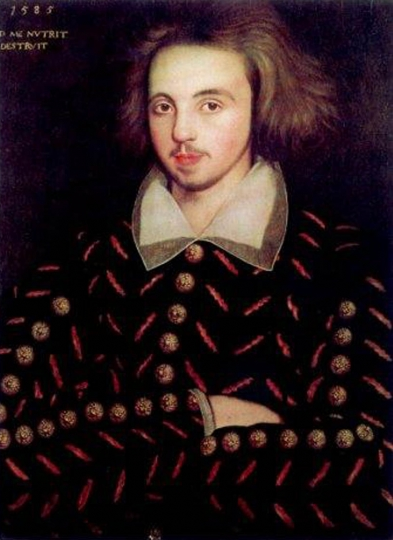
\includegraphics[height = 5 cm]{Marlowe.png}
\caption{swag}
\end{figure}

\subsection{Problematisering}
Allt som finns i skafferiet eller kylen kan inte hållas i huvudet. Det leder till att bäst före-datum glöms bort, vilket slutar med att matvaror blir för gamla och måste slängas. Samtidigt gör dålig koll på matvarorna i huset att inköpen blir svåra att planera. Detta innebär att det finns en risk att varor köps in fast de inte behövs. De hinner inte förtäras och blir dåliga. 
\noindent \newline \newline
Rapporten kommer ta upp appens uppbyggnad, dess funktioner och nytta i samhället, lokalt och globalt.


\subsection{Målsättning och syfte}
Skriva en rapport om ett nytt IT-system och beskriva dess tekniska karaktär, samt diskutera runt etiska, samhälleliga och hållbarhetsaspekter. Rapporten är även för att träna användandet av referenser och en introduktion till Urkund. 
\noindent \newline \newline
Målet med appen är att ingen mat ska behöva slängas. Detta genom ett system som fungerar som ett stöd vid planering och inventering av diverse förråd, såsom kylskåpet.

\pagebreak

\section{Resultat}


\subsection{Stora miljöproblemet med den enkla lösningen}
Detta system håller koll på dina matvaror i skafferiet, kylskåpet och frysen. Varorna inventeras i en databas du kan nå med en smartphone. I databasen lagras förutom namnet på varan: kvantitet, inköpsdatum och kategori. Detta gör att du har fullständig koll på matvarorna i hemmet. 
\noindent \newline \newline
Enligt Naturvårdsverket svarar hushåll för den största delen av mängden matavfall i Sverige. I genomsnitt slänger varje person 72 kg mat varje år. Anledningen som ges är en alltför dålig planering, vilket medför svinn. Detta visar sig i form av överinköp, feltolkning av bäst före dag, att alla delar av råvarorna inte används och att tömningen av förpackningar inte görs ordentligt.\cite{Nverket}
\noindent \newline \newline
Appen ska minska mängden slängd mat genom att simplifiera matplaneringen och hålla koll på gamla varor. Användaren kan välja i vilken grad den vill använda systemet. Det går bra att enbart använda det till planering, men det ska också finnas en funktion för att skriva in recept och därigenom beräkna portionspriser. 


\subsection{En lagerarbetare i hemmet}
Den första versionen av systemet kommer enbart vara kopplat till en matvarukedjas kundkort till exempel ICA-kortet. Allt du handlar där förs automatiskt in i databasen och det är sedan upp till dig att kategorisera dem. Det är enbart den första inmatningen av en vara som behöver göras. Sedan kommer det skötas med hjälp av dina tidigare kategoriseringar. Succesivt när du handlar så fylls din databas på och struktureras efter dina preferenser. 
\noindent \newline \newline
Någon gång kommer dock varor ta slut och då ska de flyttas ut ur databasen. Då läser du in varans streckkod med en läsare, vilket leder till att streckkoden kopplas till den scannade varan och plockas ut ur databasen. Den borttagna varan försvinner dock inte helt. Den sparas i en lista, som kan användas vid nästa handling för att lätt se vad som tagit slut.
\noindent \newline \newline
Det finns streckkodsläsare att köpa för hemmet, som kan koppla upp sig mot en dator eller smartphone med Bluetooth för att lätt inventera lager.\cite{Mynewsdesk} Vid många fall kommer dock en streckkodsläsare inte behöva inköpas. I en undersökning från juli 2012 av Flurry har 86 procent av alla svenskar mellan 15 och 64 år en smartphone.\cite{Flurry} En kamera är inkluderat i de flesta smartphones och den kan användas till att läsa streckkoder. Ett exempel är Samsungs Galaxy Round med 13 MP kamera.\cite{NyTeknik} Det finns ett flertal appar som läser streckkoder, såsom Barcode Scanner av ZXing Team och QR BARCODE SCANNER av WB Development Team.\cite{BarcodeScanner, QRBarcodeScanner} 
\noindent \newline \newline
En streckkodsläsare kommer vara inkluderad i appen, men det kommer även finnas möjligheten att ta bort varorna manuellt i listan om användaren skulle föredra det.             
\noindent \newline \newline
Appen kan även arbeta med recept. När ett recept ska matas in skriver användaren ingredienserna och mängden som ska användas, vilket leder till att programmet beräknar portionspris för varorna och maträtten. Det går även att använda streckkodsläsaren för mata in varorna för ett recept. Receptinmatningen är ett verktyg för att hjälpa till med matbudgeten och på ett enkelt sätt visa vilka komponenter i maträtten som är dyrast.        


\subsection{Gör som andra fast bättre}
Det finns flera inventarieprogram på marknaden. En av dem är The Home Food Storage App för iOS. Den låter dig scanna in varorna. Alltså, för varje handling måste du föra in alla varor i systemet. Inköpslista är integrerat och även mål för hur länge varor ska räcka. -Den håller också koll på bäst före-datumet.\cite{FoodStorageApp} 
\noindent \newline \newline
En liknande produkt för smartphones med Android heter Inventory Droid och även den använder sig av telefonens kamera för att skanna streckkoder. Databasen du bygger upp kan lätt exporteras till Excel för lättare bearbetning, vilket gör övergång från smartphone till dator väldigt användarvänligt. Den mer avancerade användaren kan manipulera Exceldokumentet för att beräkna portionspris och dylikt.\cite{InventoryDroid} 


\subsection{Visioner för framtiden}
Appen ska i framtiden samarbeta med de flesta matbutikerna i Sverige. Du ska kunna handla överallt och ändå ha koll på skafferiet hemma. 
\noindent \newline \newline
Findity AB arbetar för att butiker ska lämna ut digitala kvitton som du enkelt har tillgång till genom en smartphone eller dator.\cite{SparaKvittot} Digitalisering av kvitton gör det lättare för den beskrivna appen att spridas, eftersom det då kan baseras på det digitala kvittosystemet.
\noindent \newline \newline
När systemet slagit igenom i Sverige kan det expandera till Europa och sedan världen.            

\pagebreak

\section{Diskussion}
För att appen ska användas krävs det otrolig användarvänlighet. Det får inte vara svårt att manipulera informationen i databasen. Att använda sig av inventerieappar är inte särskilt utspritt och jag tror att det beror på den oerhörda tiden det tar att uppdatera databasen. Den beskrivna appen i rapporten automatiserar det mest tidskrävande steget, vilket är att mata in varor i databasen.
\noindent \newline \newline
Det som krävs för att appen ska bli verklighet är ett samarbete med en stor matvarukedja eller ett vidsträckt system med digitala kvitton. Det som ligger närmast framtiden är förmodligen ett samarbete med en matvarukedja. Tyvärr kan det medföra att matvarukedjan ifråga vill vara unika med systemet och därmed förhindrar spridning, men det kan vara nödvändigt för att få ut appen. Det optimala är en internationell utbredning, vilket skulle medföra att den oerhörda mängden slängd mat skulle minska.
\noindent \newline \newline
Appen är anpassat för moderna smartphones med inbyggd kamera och det är där själva målgruppen finns.  Dock förhindrar detta att systemet får en större spridning i områden utan den levnadsstandarden. De har kanske inte heller samma problem med överinköp. Det är alltså främst  i-länder som är marknaden. 
\noindent \newline \newline
Varje gång man slänger mat så slösar man på ekonomi, miljö och även etik. I-länder slänger mat medan människor i andra länder inte har mat på bordet. Det är inte etiskt rimligt och det är ännu en anledning till varför appen borde finnas. Även om du måste lägga ned tid på att kategorisera databasen från början och ta bort varor ur databasen när de är slut, kan den tiden vara värd det. Då gör du skillnad. 

  


\pagebreak
\begin{thebibliography}{references}

\bibitem{NyTeknik}
Abrahamsson, Håkan. (2013). 	
Koreaner visar upp sin krökta mobil. Nyteknik, 16 oktober, 42, s. 18.

\bibitem{Mynewsdesk}
Amini, Khazar. My News Desk. "Smidig streckkodsläsare löser dina problem". \url{http://www.mynewsdesk.com/se/deltaco-ab/pressreleases/smidig-streckkodslaesare-loeser-dina-problem-876374}.[Hämtad den 2013-10-22].

\bibitem{QRBarcodeScanner}
Google play. WB Development Team. "QR BARCODE SCANNER". \url{https://play.google.com/store/apps/details?id=appinventor.ai_progetto2003.SCAN&hl=sv}[Hämtad den 2013-10-20]

\bibitem{BarcodeScanner}
Google play. ZXing Team. "Barcode Scanner". \url{https://play.google.com/store/apps/details?id=com.google.zxing.client.android&hl=sv}[Hämtad 2013-10-20]

\bibitem{SparaKvittot}
Findity AB. Sparakvittot. "Om Sparakvittot". \url{http://www.sparakvittot.se/om-sparakvittot}[Hämtad 2013-10-22].

\bibitem{Flurry}
Flurry. Flurry Blog. "iOS and Android Adoption Explodes Internationally". \url{http://blog.flurry.com//bid/88867/ios-and-android-adoption-explodes-internationally}[Hämtad den 2013-10-20].

\bibitem{FoodStorageApp}
Long Term Glass Wares LLC. The Home Food Storage App. \url{http://www.foodstorageapp.com/}[Hämtad den 2013-10-19].

\bibitem{InventoryDroid}
RomiSys. Inventory Droid. \url{http://www.romisys.com/pages/inventory-droid.php}.[Hämtad 2013-10-22].
  
\bibitem{Nverket}
Sjöström, Sanna. Naturvårdsverket. "Matsvinn".
\url{http://www.naturvardsverket.se/Miljoarbete-i-samhallet/Miljoarbete-i-Sverige/Uppdelat-efter-omrade/Avfall/Avfallsforebyggande-program/Mat/}[Hämtad den 2013-10-19].





\end{thebibliography}

\end{document}
\documentclass[12pt, a4paper]{article}
\usepackage[swedish]{babel}
\usepackage[utf8]{inputenc}
\usepackage{fullpage}
\usepackage{graphicx}
\usepackage{hyperref}
\usepackage[nottoc,numbib]{tocbibind}
\title{Vad har jag i kylen egentligen?}
\author{Adam Vendelin}


\begin{document}
\maketitle
\begin{center}Uppsala Universitet 
\end{center}
\begin{center}2013-10-24
\end{center}
\pagebreak
\tableofcontents
\pagebreak

\section{Sammanfattning}
\begin{center} \parbox{12cm}{Rapporten behandlar en app som hjälper dig vid inventering av kylskåp och skafferier. Det gör att risken för överinköp minskar, vilket är bra för miljön, ekonomin och även på ett etiskt sätt.  \newline \newline \textit{Nyckelord:}app, databas, inventering, miljö.}
\end{center}
\pagebreak


\section{Introduktion}
\subsection{Bakgrund}
Den här rapporten presenterar en app, utvecklat för att hjälpa människor och miljön. Du ska enkelt kunna se vad som finns i kylskåpet och skafferiet utan att behöva öppna dörrar eller ens vara i huset. Allt detta utan att behöva lägga ned mycket tid på inventeringen. 

\begin{figure}[h!]
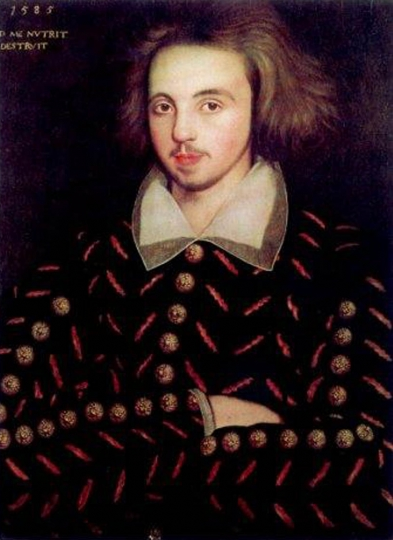
\includegraphics[height = 5 cm]{Marlowe.jpg}
\caption{swag}
\end{figure}

\subsection{Problematisering}
Allt som finns i skafferiet eller kylen kan inte hållas i huvudet. Det leder till att bäst före-datum glöms bort, vilket slutar med att matvaror blir för gamla och måste slängas. Samtidigt gör dålig koll på matvarorna i huset att inköpen blir svåra att planera. Detta innebär att det finns en risk att varor köps in fast de inte behövs. De hinner inte förtäras och blir dåliga. 
\noindent \newline \newline
Rapporten kommer ta upp appens uppbyggnad, dess funktioner och nytta i samhället, lokalt och globalt.


\subsection{Målsättning och syfte}
Skriva en rapport om ett nytt IT-system och beskriva dess tekniska karaktär, samt diskutera runt etiska, samhälleliga och hållbarhetsaspekter. Rapporten är även för att träna användandet av referenser och en introduktion till Urkund. 
\noindent \newline \newline
Målet med appen är att ingen mat ska behöva slängas. Detta genom ett system som fungerar som ett stöd vid planering och inventering av diverse förråd, såsom kylskåpet.

\pagebreak

\section{Resultat}


\subsection{Stora miljöproblemet med den enkla lösningen}
Detta system håller koll på dina matvaror i skafferiet, kylskåpet och frysen. Varorna inventeras i en databas du kan nå med en smartphone. I databasen lagras förutom namnet på varan: kvantitet, inköpsdatum och kategori. Detta gör att du har fullständig koll på matvarorna i hemmet. 
\noindent \newline \newline
Enligt Naturvårdsverket svarar hushåll för den största delen av mängden matavfall i Sverige. I genomsnitt slänger varje person 72 kg mat varje år. Anledningen som ges är en alltför dålig planering, vilket medför svinn. Detta visar sig i form av överinköp, feltolkning av bäst före dag, att alla delar av råvarorna inte används och att tömningen av förpackningar inte görs ordentligt.\cite{Nverket}
\noindent \newline \newline
Appen ska minska mängden slängd mat genom att simplifiera matplaneringen och hålla koll på gamla varor. Användaren kan välja i vilken grad den vill använda systemet. Det går bra att enbart använda det till planering, men det ska också finnas en funktion för att skriva in recept och därigenom beräkna portionspriser. 


\subsection{En lagerarbetare i hemmet}
Den första versionen av systemet kommer enbart vara kopplat till en matvarukedjas kundkort till exempel ICA-kortet. Allt du handlar där förs automatiskt in i databasen och det är sedan upp till dig att kategorisera dem. Det är enbart den första inmatningen av en vara som behöver göras. Sedan kommer det skötas med hjälp av dina tidigare kategoriseringar. Succesivt när du handlar så fylls din databas på och struktureras efter dina preferenser. 
\noindent \newline \newline
Någon gång kommer dock varor ta slut och då ska de flyttas ut ur databasen. Då läser du in varans streckkod med en läsare, vilket leder till att streckkoden kopplas till den scannade varan och plockas ut ur databasen. Den borttagna varan försvinner dock inte helt. Den sparas i en lista, som kan användas vid nästa handling för att lätt se vad som tagit slut.
\noindent \newline \newline
Det finns streckkodsläsare att köpa för hemmet, som kan koppla upp sig mot en dator eller smartphone med Bluetooth för att lätt inventera lager.\cite{Mynewsdesk} Vid många fall kommer dock en streckkodsläsare inte behöva inköpas. I en undersökning från juli 2012 av Flurry har 86 procent av alla svenskar mellan 15 och 64 år en smartphone.\cite{Flurry} En kamera är inkluderat i de flesta smartphones och den kan användas till att läsa streckkoder. Ett exempel är Samsungs Galaxy Round med 13 MP kamera.\cite{NyTeknik} Det finns ett flertal appar som läser streckkoder, såsom Barcode Scanner av ZXing Team och QR BARCODE SCANNER av WB Development Team.\cite{BarcodeScanner, QRBarcodeScanner} 
\noindent \newline \newline
En streckkodsläsare kommer vara inkluderad i appen, men det kommer även finnas möjligheten att ta bort varorna manuellt i listan om användaren skulle föredra det.             
\noindent \newline \newline
Appen kan även arbeta med recept. När ett recept ska matas in skriver användaren ingredienserna och mängden som ska användas, vilket leder till att programmet beräknar portionspris för varorna och maträtten. Det går även att använda streckkodsläsaren för mata in varorna för ett recept. Receptinmatningen är ett verktyg för att hjälpa till med matbudgeten och på ett enkelt sätt visa vilka komponenter i maträtten som är dyrast.        


\subsection{Gör som andra fast bättre}
Det finns flera inventarieprogram på marknaden. En av dem är The Home Food Storage App för iOS. Den låter dig scanna in varorna. Alltså, för varje handling måste du föra in alla varor i systemet. Inköpslista är integrerat och även mål för hur länge varor ska räcka. -Den håller också koll på bäst före-datumet.\cite{FoodStorageApp} 
\noindent \newline \newline
En liknande produkt för smartphones med Android heter Inventory Droid och även den använder sig av telefonens kamera för att skanna streckkoder. Databasen du bygger upp kan lätt exporteras till Excel för lättare bearbetning, vilket gör övergång från smartphone till dator väldigt användarvänligt. Den mer avancerade användaren kan manipulera Exceldokumentet för att beräkna portionspris och dylikt.\cite{InventoryDroid} 


\subsection{Visioner för framtiden}
Appen ska i framtiden samarbeta med de flesta matbutikerna i Sverige. Du ska kunna handla överallt och ändå ha koll på skafferiet hemma. 
\noindent \newline \newline
Findity AB arbetar för att butiker ska lämna ut digitala kvitton som du enkelt har tillgång till genom en smartphone eller dator.\cite{SparaKvittot} Digitalisering av kvitton gör det lättare för den beskrivna appen att spridas, eftersom det då kan baseras på det digitala kvittosystemet.
\noindent \newline \newline
När systemet slagit igenom i Sverige kan det expandera till Europa och sedan världen.            

\pagebreak

\section{Diskussion}
För att appen ska användas krävs det otrolig användarvänlighet. Det får inte vara svårt att manipulera informationen i databasen. Att använda sig av inventerieappar är inte särskilt utspritt och jag tror att det beror på den oerhörda tiden det tar att uppdatera databasen. Den beskrivna appen i rapporten automatiserar det mest tidskrävande steget, vilket är att mata in varor i databasen.
\noindent \newline \newline
Det som krävs för att appen ska bli verklighet är ett samarbete med en stor matvarukedja eller ett vidsträckt system med digitala kvitton. Det som ligger närmast framtiden är förmodligen ett samarbete med en matvarukedja. Tyvärr kan det medföra att matvarukedjan ifråga vill vara unika med systemet och därmed förhindrar spridning, men det kan vara nödvändigt för att få ut appen. Det optimala är en internationell utbredning, vilket skulle medföra att den oerhörda mängden slängd mat skulle minska.
\noindent \newline \newline
Appen är anpassat för moderna smartphones med inbyggd kamera och det är där själva målgruppen finns.  Dock förhindrar detta att systemet får en större spridning i områden utan den levnadsstandarden. De har kanske inte heller samma problem med överinköp. Det är alltså främst  i-länder som är marknaden. 
\noindent \newline \newline
Varje gång man slänger mat så slösar man på ekonomi, miljö och även etik. I-länder slänger mat medan människor i andra länder inte har mat på bordet. Det är inte etiskt rimligt och det är ännu en anledning till varför appen borde finnas. Även om du måste lägga ned tid på att kategorisera databasen från början och ta bort varor ur databasen när de är slut, kan den tiden vara värd det. Då gör du skillnad. 

  


\pagebreak
\begin{thebibliography}{references}

\bibitem{NyTeknik}
Abrahamsson, Håkan. (2013). 	
Koreaner visar upp sin krökta mobil. Nyteknik, 16 oktober, 42, s. 18.

\bibitem{Mynewsdesk}
Amini, Khazar. My News Desk. "Smidig streckkodsläsare löser dina problem". \url{http://www.mynewsdesk.com/se/deltaco-ab/pressreleases/smidig-streckkodslaesare-loeser-dina-problem-876374}.[Hämtad den 2013-10-22].

\bibitem{QRBarcodeScanner}
Google play. WB Development Team. "QR BARCODE SCANNER". \url{https://play.google.com/store/apps/details?id=appinventor.ai_progetto2003.SCAN&hl=sv}[Hämtad den 2013-10-20]

\bibitem{BarcodeScanner}
Google play. ZXing Team. "Barcode Scanner". \url{https://play.google.com/store/apps/details?id=com.google.zxing.client.android&hl=sv}[Hämtad 2013-10-20]

\bibitem{SparaKvittot}
Findity AB. Sparakvittot. "Om Sparakvittot". \url{http://www.sparakvittot.se/om-sparakvittot}[Hämtad 2013-10-22].

\bibitem{Flurry}
Flurry. Flurry Blog. "iOS and Android Adoption Explodes Internationally". \url{http://blog.flurry.com//bid/88867/ios-and-android-adoption-explodes-internationally}[Hämtad den 2013-10-20].

\bibitem{FoodStorageApp}
Long Term Glass Wares LLC. The Home Food Storage App. \url{http://www.foodstorageapp.com/}[Hämtad den 2013-10-19].

\bibitem{InventoryDroid}
RomiSys. Inventory Droid. \url{http://www.romisys.com/pages/inventory-droid.php}.[Hämtad 2013-10-22].
  
\bibitem{Nverket}
Sjöström, Sanna. Naturvårdsverket. "Matsvinn".
\url{http://www.naturvardsverket.se/Miljoarbete-i-samhallet/Miljoarbete-i-Sverige/Uppdelat-efter-omrade/Avfall/Avfallsforebyggande-program/Mat/}[Hämtad den 2013-10-19].





\end{thebibliography}

\end{document}
\documentclass[12pt, a4paper]{article}
\usepackage[swedish]{babel}
\usepackage[utf8]{inputenc}
\usepackage{fullpage}
\usepackage{graphicx}
\usepackage{hyperref}
\usepackage[nottoc,numbib]{tocbibind}
\title{Vad har jag i kylen egentligen?}
\author{Adam Vendelin}


\begin{document}
\maketitle
\begin{center}Uppsala Universitet 
\end{center}
\begin{center}2013-10-24
\end{center}
\pagebreak
\tableofcontents
\pagebreak

\section{Sammanfattning}
\begin{center} \parbox{12cm}{Rapporten behandlar en app som hjälper dig vid inventering av kylskåp och skafferier. Det gör att risken för överinköp minskar, vilket är bra för miljön, ekonomin och även på ett etiskt sätt.  \newline \newline \textit{Nyckelord:}app, databas, inventering, miljö.}
\end{center}
\pagebreak


\section{Introduktion}
\subsection{Bakgrund}
Den här rapporten presenterar en app, utvecklat för att hjälpa människor och miljön. Du ska enkelt kunna se vad som finns i kylskåpet och skafferiet utan att behöva öppna dörrar eller ens vara i huset. Allt detta utan att behöva lägga ned mycket tid på inventeringen. 

\begin{figure}[h!]
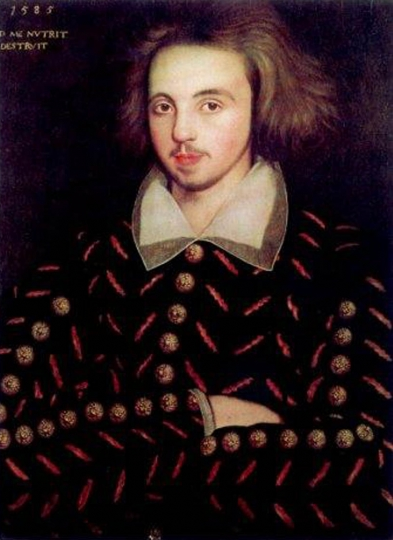
\includegraphics[height = 5 cm]{Marlowe.jpg}
\caption{swag}
\end{figure}

\subsection{Problematisering}
Allt som finns i skafferiet eller kylen kan inte hållas i huvudet. Det leder till att bäst före-datum glöms bort, vilket slutar med att matvaror blir för gamla och måste slängas. Samtidigt gör dålig koll på matvarorna i huset att inköpen blir svåra att planera. Detta innebär att det finns en risk att varor köps in fast de inte behövs. De hinner inte förtäras och blir dåliga. 
\noindent \newline \newline
Rapporten kommer ta upp appens uppbyggnad, dess funktioner och nytta i samhället, lokalt och globalt.


\subsection{Målsättning och syfte}
Skriva en rapport om ett nytt IT-system och beskriva dess tekniska karaktär, samt diskutera runt etiska, samhälleliga och hållbarhetsaspekter. Rapporten är även för att träna användandet av referenser och en introduktion till Urkund. 
\noindent \newline \newline
Målet med appen är att ingen mat ska behöva slängas. Detta genom ett system som fungerar som ett stöd vid planering och inventering av diverse förråd, såsom kylskåpet.

\pagebreak

\section{Resultat}


\subsection{Stora miljöproblemet med den enkla lösningen}
Detta system håller koll på dina matvaror i skafferiet, kylskåpet och frysen. Varorna inventeras i en databas du kan nå med en smartphone. I databasen lagras förutom namnet på varan: kvantitet, inköpsdatum och kategori. Detta gör att du har fullständig koll på matvarorna i hemmet. 
\noindent \newline \newline
Enligt Naturvårdsverket svarar hushåll för den största delen av mängden matavfall i Sverige. I genomsnitt slänger varje person 72 kg mat varje år. Anledningen som ges är en alltför dålig planering, vilket medför svinn. Detta visar sig i form av överinköp, feltolkning av bäst före dag, att alla delar av råvarorna inte används och att tömningen av förpackningar inte görs ordentligt.\cite{Nverket}
\noindent \newline \newline
Appen ska minska mängden slängd mat genom att simplifiera matplaneringen och hålla koll på gamla varor. Användaren kan välja i vilken grad den vill använda systemet. Det går bra att enbart använda det till planering, men det ska också finnas en funktion för att skriva in recept och därigenom beräkna portionspriser. 


\subsection{En lagerarbetare i hemmet}
Den första versionen av systemet kommer enbart vara kopplat till en matvarukedjas kundkort till exempel ICA-kortet. Allt du handlar där förs automatiskt in i databasen och det är sedan upp till dig att kategorisera dem. Det är enbart den första inmatningen av en vara som behöver göras. Sedan kommer det skötas med hjälp av dina tidigare kategoriseringar. Succesivt när du handlar så fylls din databas på och struktureras efter dina preferenser. 
\noindent \newline \newline
Någon gång kommer dock varor ta slut och då ska de flyttas ut ur databasen. Då läser du in varans streckkod med en läsare, vilket leder till att streckkoden kopplas till den scannade varan och plockas ut ur databasen. Den borttagna varan försvinner dock inte helt. Den sparas i en lista, som kan användas vid nästa handling för att lätt se vad som tagit slut.
\noindent \newline \newline
Det finns streckkodsläsare att köpa för hemmet, som kan koppla upp sig mot en dator eller smartphone med Bluetooth för att lätt inventera lager.\cite{Mynewsdesk} Vid många fall kommer dock en streckkodsläsare inte behöva inköpas. I en undersökning från juli 2012 av Flurry har 86 procent av alla svenskar mellan 15 och 64 år en smartphone.\cite{Flurry} En kamera är inkluderat i de flesta smartphones och den kan användas till att läsa streckkoder. Ett exempel är Samsungs Galaxy Round med 13 MP kamera.\cite{NyTeknik} Det finns ett flertal appar som läser streckkoder, såsom Barcode Scanner av ZXing Team och QR BARCODE SCANNER av WB Development Team.\cite{BarcodeScanner, QRBarcodeScanner} 
\noindent \newline \newline
En streckkodsläsare kommer vara inkluderad i appen, men det kommer även finnas möjligheten att ta bort varorna manuellt i listan om användaren skulle föredra det.             
\noindent \newline \newline
Appen kan även arbeta med recept. När ett recept ska matas in skriver användaren ingredienserna och mängden som ska användas, vilket leder till att programmet beräknar portionspris för varorna och maträtten. Det går även att använda streckkodsläsaren för mata in varorna för ett recept. Receptinmatningen är ett verktyg för att hjälpa till med matbudgeten och på ett enkelt sätt visa vilka komponenter i maträtten som är dyrast.        


\subsection{Gör som andra fast bättre}
Det finns flera inventarieprogram på marknaden. En av dem är The Home Food Storage App för iOS. Den låter dig scanna in varorna. Alltså, för varje handling måste du föra in alla varor i systemet. Inköpslista är integrerat och även mål för hur länge varor ska räcka. -Den håller också koll på bäst före-datumet.\cite{FoodStorageApp} 
\noindent \newline \newline
En liknande produkt för smartphones med Android heter Inventory Droid och även den använder sig av telefonens kamera för att skanna streckkoder. Databasen du bygger upp kan lätt exporteras till Excel för lättare bearbetning, vilket gör övergång från smartphone till dator väldigt användarvänligt. Den mer avancerade användaren kan manipulera Exceldokumentet för att beräkna portionspris och dylikt.\cite{InventoryDroid} 


\subsection{Visioner för framtiden}
Appen ska i framtiden samarbeta med de flesta matbutikerna i Sverige. Du ska kunna handla överallt och ändå ha koll på skafferiet hemma. 
\noindent \newline \newline
Findity AB arbetar för att butiker ska lämna ut digitala kvitton som du enkelt har tillgång till genom en smartphone eller dator.\cite{SparaKvittot} Digitalisering av kvitton gör det lättare för den beskrivna appen att spridas, eftersom det då kan baseras på det digitala kvittosystemet.
\noindent \newline \newline
När systemet slagit igenom i Sverige kan det expandera till Europa och sedan världen.            

\pagebreak

\section{Diskussion}
För att appen ska användas krävs det otrolig användarvänlighet. Det får inte vara svårt att manipulera informationen i databasen. Att använda sig av inventerieappar är inte särskilt utspritt och jag tror att det beror på den oerhörda tiden det tar att uppdatera databasen. Den beskrivna appen i rapporten automatiserar det mest tidskrävande steget, vilket är att mata in varor i databasen.
\noindent \newline \newline
Det som krävs för att appen ska bli verklighet är ett samarbete med en stor matvarukedja eller ett vidsträckt system med digitala kvitton. Det som ligger närmast framtiden är förmodligen ett samarbete med en matvarukedja. Tyvärr kan det medföra att matvarukedjan ifråga vill vara unika med systemet och därmed förhindrar spridning, men det kan vara nödvändigt för att få ut appen. Det optimala är en internationell utbredning, vilket skulle medföra att den oerhörda mängden slängd mat skulle minska.
\noindent \newline \newline
Appen är anpassat för moderna smartphones med inbyggd kamera och det är där själva målgruppen finns.  Dock förhindrar detta att systemet får en större spridning i områden utan den levnadsstandarden. De har kanske inte heller samma problem med överinköp. Det är alltså främst  i-länder som är marknaden. 
\noindent \newline \newline
Varje gång man slänger mat så slösar man på ekonomi, miljö och även etik. I-länder slänger mat medan människor i andra länder inte har mat på bordet. Det är inte etiskt rimligt och det är ännu en anledning till varför appen borde finnas. Även om du måste lägga ned tid på att kategorisera databasen från början och ta bort varor ur databasen när de är slut, kan den tiden vara värd det. Då gör du skillnad. 

  


\pagebreak
\begin{thebibliography}{references}

\bibitem{NyTeknik}
Abrahamsson, Håkan. (2013). 	
Koreaner visar upp sin krökta mobil. Nyteknik, 16 oktober, 42, s. 18.

\bibitem{Mynewsdesk}
Amini, Khazar. My News Desk. "Smidig streckkodsläsare löser dina problem". \url{http://www.mynewsdesk.com/se/deltaco-ab/pressreleases/smidig-streckkodslaesare-loeser-dina-problem-876374}.[Hämtad den 2013-10-22].

\bibitem{QRBarcodeScanner}
Google play. WB Development Team. "QR BARCODE SCANNER". \url{https://play.google.com/store/apps/details?id=appinventor.ai_progetto2003.SCAN&hl=sv}[Hämtad den 2013-10-20]

\bibitem{BarcodeScanner}
Google play. ZXing Team. "Barcode Scanner". \url{https://play.google.com/store/apps/details?id=com.google.zxing.client.android&hl=sv}[Hämtad 2013-10-20]

\bibitem{SparaKvittot}
Findity AB. Sparakvittot. "Om Sparakvittot". \url{http://www.sparakvittot.se/om-sparakvittot}[Hämtad 2013-10-22].

\bibitem{Flurry}
Flurry. Flurry Blog. "iOS and Android Adoption Explodes Internationally". \url{http://blog.flurry.com//bid/88867/ios-and-android-adoption-explodes-internationally}[Hämtad den 2013-10-20].

\bibitem{FoodStorageApp}
Long Term Glass Wares LLC. The Home Food Storage App. \url{http://www.foodstorageapp.com/}[Hämtad den 2013-10-19].

\bibitem{InventoryDroid}
RomiSys. Inventory Droid. \url{http://www.romisys.com/pages/inventory-droid.php}.[Hämtad 2013-10-22].
  
\bibitem{Nverket}
Sjöström, Sanna. Naturvårdsverket. "Matsvinn".
\url{http://www.naturvardsverket.se/Miljoarbete-i-samhallet/Miljoarbete-i-Sverige/Uppdelat-efter-omrade/Avfall/Avfallsforebyggande-program/Mat/}[Hämtad den 2013-10-19].





\end{thebibliography}

\end{document}

\documentclass[12pt, a4paper]{article}
\usepackage[swedish]{babel}
\usepackage[utf8]{inputenc}
\usepackage{fullpage}
\usepackage{graphicx}
\usepackage{hyperref}
\usepackage[nottoc,numbib]{tocbibind}
\title{Vad har jag i kylen egentligen?}
\author{Adam Vendelin}


\begin{document}
\maketitle
\begin{center}Uppsala Universitet 
\end{center}
\begin{center}2013-10-24
\end{center}
\pagebreak
\tableofcontents
\pagebreak

\section{Sammanfattning}
\begin{center} \parbox{12cm}{Rapporten behandlar en app som hjälper dig vid inventering av kylskåp och skafferier. Det gör att risken för överinköp minskar, vilket är bra för miljön, ekonomin och även på ett etiskt sätt.  \newline \newline \textit{Nyckelord:}app, databas, inventering, miljö.}
\end{center}
\pagebreak


\section{Introduktion}
\subsection{Bakgrund}
Den här rapporten presenterar en app, utvecklat för att hjälpa människor och miljön. Du ska enkelt kunna se vad som finns i kylskåpet och skafferiet utan att behöva öppna dörrar eller ens vara i huset. Allt detta utan att behöva lägga ned mycket tid på inventeringen. 

\begin{figure}[h!]
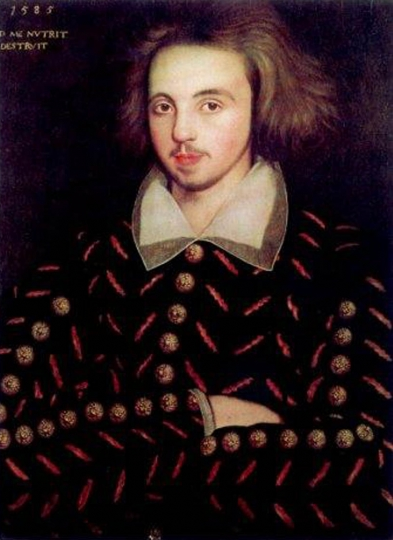
\includegraphics[height = 5 cm]{Marlowe.jpg}
\caption{swag}
\end{figure}

\subsection{Problematisering}
Allt som finns i skafferiet eller kylen kan inte hållas i huvudet. Det leder till att bäst före-datum glöms bort, vilket slutar med att matvaror blir för gamla och måste slängas. Samtidigt gör dålig koll på matvarorna i huset att inköpen blir svåra att planera. Detta innebär att det finns en risk att varor köps in fast de inte behövs. De hinner inte förtäras och blir dåliga. 
\noindent \newline \newline
Rapporten kommer ta upp appens uppbyggnad, dess funktioner och nytta i samhället, lokalt och globalt.


\subsection{Målsättning och syfte}
Skriva en rapport om ett nytt IT-system och beskriva dess tekniska karaktär, samt diskutera runt etiska, samhälleliga och hållbarhetsaspekter. Rapporten är även för att träna användandet av referenser och en introduktion till Urkund. 
\noindent \newline \newline
Målet med appen är att ingen mat ska behöva slängas. Detta genom ett system som fungerar som ett stöd vid planering och inventering av diverse förråd, såsom kylskåpet.

\pagebreak

\section{Resultat}


\subsection{Stora miljöproblemet med den enkla lösningen}
Detta system håller koll på dina matvaror i skafferiet, kylskåpet och frysen. Varorna inventeras i en databas du kan nå med en smartphone. I databasen lagras förutom namnet på varan: kvantitet, inköpsdatum och kategori. Detta gör att du har fullständig koll på matvarorna i hemmet. 
\noindent \newline \newline
Enligt Naturvårdsverket svarar hushåll för den största delen av mängden matavfall i Sverige. I genomsnitt slänger varje person 72 kg mat varje år. Anledningen som ges är en alltför dålig planering, vilket medför svinn. Detta visar sig i form av överinköp, feltolkning av bäst före dag, att alla delar av råvarorna inte används och att tömningen av förpackningar inte görs ordentligt.\cite{Nverket}
\noindent \newline \newline
Appen ska minska mängden slängd mat genom att simplifiera matplaneringen och hålla koll på gamla varor. Användaren kan välja i vilken grad den vill använda systemet. Det går bra att enbart använda det till planering, men det ska också finnas en funktion för att skriva in recept och därigenom beräkna portionspriser. 


\subsection{En lagerarbetare i hemmet}
Den första versionen av systemet kommer enbart vara kopplat till en matvarukedjas kundkort till exempel ICA-kortet. Allt du handlar där förs automatiskt in i databasen och det är sedan upp till dig att kategorisera dem. Det är enbart den första inmatningen av en vara som behöver göras. Sedan kommer det skötas med hjälp av dina tidigare kategoriseringar. Succesivt när du handlar så fylls din databas på och struktureras efter dina preferenser. 
\noindent \newline \newline
Någon gång kommer dock varor ta slut och då ska de flyttas ut ur databasen. Då läser du in varans streckkod med en läsare, vilket leder till att streckkoden kopplas till den scannade varan och plockas ut ur databasen. Den borttagna varan försvinner dock inte helt. Den sparas i en lista, som kan användas vid nästa handling för att lätt se vad som tagit slut.
\noindent \newline \newline
Det finns streckkodsläsare att köpa för hemmet, som kan koppla upp sig mot en dator eller smartphone med Bluetooth för att lätt inventera lager.\cite{Mynewsdesk} Vid många fall kommer dock en streckkodsläsare inte behöva inköpas. I en undersökning från juli 2012 av Flurry har 86 procent av alla svenskar mellan 15 och 64 år en smartphone.\cite{Flurry} En kamera är inkluderat i de flesta smartphones och den kan användas till att läsa streckkoder. Ett exempel är Samsungs Galaxy Round med 13 MP kamera.\cite{NyTeknik} Det finns ett flertal appar som läser streckkoder, såsom Barcode Scanner av ZXing Team och QR BARCODE SCANNER av WB Development Team.\cite{BarcodeScanner, QRBarcodeScanner} 
\noindent \newline \newline
En streckkodsläsare kommer vara inkluderad i appen, men det kommer även finnas möjligheten att ta bort varorna manuellt i listan om användaren skulle föredra det.             
\noindent \newline \newline
Appen kan även arbeta med recept. När ett recept ska matas in skriver användaren ingredienserna och mängden som ska användas, vilket leder till att programmet beräknar portionspris för varorna och maträtten. Det går även att använda streckkodsläsaren för mata in varorna för ett recept. Receptinmatningen är ett verktyg för att hjälpa till med matbudgeten och på ett enkelt sätt visa vilka komponenter i maträtten som är dyrast.        


\subsection{Gör som andra fast bättre}
Det finns flera inventarieprogram på marknaden. En av dem är The Home Food Storage App för iOS. Den låter dig scanna in varorna. Alltså, för varje handling måste du föra in alla varor i systemet. Inköpslista är integrerat och även mål för hur länge varor ska räcka. -Den håller också koll på bäst före-datumet.\cite{FoodStorageApp} 
\noindent \newline \newline
En liknande produkt för smartphones med Android heter Inventory Droid och även den använder sig av telefonens kamera för att skanna streckkoder. Databasen du bygger upp kan lätt exporteras till Excel för lättare bearbetning, vilket gör övergång från smartphone till dator väldigt användarvänligt. Den mer avancerade användaren kan manipulera Exceldokumentet för att beräkna portionspris och dylikt.\cite{InventoryDroid} 


\subsection{Visioner för framtiden}
Appen ska i framtiden samarbeta med de flesta matbutikerna i Sverige. Du ska kunna handla överallt och ändå ha koll på skafferiet hemma. 
\noindent \newline \newline
Findity AB arbetar för att butiker ska lämna ut digitala kvitton som du enkelt har tillgång till genom en smartphone eller dator.\cite{SparaKvittot} Digitalisering av kvitton gör det lättare för den beskrivna appen att spridas, eftersom det då kan baseras på det digitala kvittosystemet.
\noindent \newline \newline
När systemet slagit igenom i Sverige kan det expandera till Europa och sedan världen.            

\pagebreak

\section{Diskussion}
För att appen ska användas krävs det otrolig användarvänlighet. Det får inte vara svårt att manipulera informationen i databasen. Att använda sig av inventerieappar är inte särskilt utspritt och jag tror att det beror på den oerhörda tiden det tar att uppdatera databasen. Den beskrivna appen i rapporten automatiserar det mest tidskrävande steget, vilket är att mata in varor i databasen.
\noindent \newline \newline
Det som krävs för att appen ska bli verklighet är ett samarbete med en stor matvarukedja eller ett vidsträckt system med digitala kvitton. Det som ligger närmast framtiden är förmodligen ett samarbete med en matvarukedja. Tyvärr kan det medföra att matvarukedjan ifråga vill vara unika med systemet och därmed förhindrar spridning, men det kan vara nödvändigt för att få ut appen. Det optimala är en internationell utbredning, vilket skulle medföra att den oerhörda mängden slängd mat skulle minska.
\noindent \newline \newline
Appen är anpassat för moderna smartphones med inbyggd kamera och det är där själva målgruppen finns.  Dock förhindrar detta att systemet får en större spridning i områden utan den levnadsstandarden. De har kanske inte heller samma problem med överinköp. Det är alltså främst  i-länder som är marknaden. 
\noindent \newline \newline
Varje gång man slänger mat så slösar man på ekonomi, miljö och även etik. I-länder slänger mat medan människor i andra länder inte har mat på bordet. Det är inte etiskt rimligt och det är ännu en anledning till varför appen borde finnas. Även om du måste lägga ned tid på att kategorisera databasen från början och ta bort varor ur databasen när de är slut, kan den tiden vara värd det. Då gör du skillnad. 

  


\pagebreak
\begin{thebibliography}{references}

\bibitem{NyTeknik}
Abrahamsson, Håkan. (2013). 	
Koreaner visar upp sin krökta mobil. Nyteknik, 16 oktober, 42, s. 18.

\bibitem{Mynewsdesk}
Amini, Khazar. My News Desk. "Smidig streckkodsläsare löser dina problem". \url{http://www.mynewsdesk.com/se/deltaco-ab/pressreleases/smidig-streckkodslaesare-loeser-dina-problem-876374}.[Hämtad den 2013-10-22].

\bibitem{QRBarcodeScanner}
Google play. WB Development Team. "QR BARCODE SCANNER". \url{https://play.google.com/store/apps/details?id=appinventor.ai_progetto2003.SCAN&hl=sv}[Hämtad den 2013-10-20]

\bibitem{BarcodeScanner}
Google play. ZXing Team. "Barcode Scanner". \url{https://play.google.com/store/apps/details?id=com.google.zxing.client.android&hl=sv}[Hämtad 2013-10-20]

\bibitem{SparaKvittot}
Findity AB. Sparakvittot. "Om Sparakvittot". \url{http://www.sparakvittot.se/om-sparakvittot}[Hämtad 2013-10-22].

\bibitem{Flurry}
Flurry. Flurry Blog. "iOS and Android Adoption Explodes Internationally". \url{http://blog.flurry.com//bid/88867/ios-and-android-adoption-explodes-internationally}[Hämtad den 2013-10-20].

\bibitem{FoodStorageApp}
Long Term Glass Wares LLC. The Home Food Storage App. \url{http://www.foodstorageapp.com/}[Hämtad den 2013-10-19].

\bibitem{InventoryDroid}
RomiSys. Inventory Droid. \url{http://www.romisys.com/pages/inventory-droid.php}.[Hämtad 2013-10-22].
  
\bibitem{Nverket}
Sjöström, Sanna. Naturvårdsverket. "Matsvinn".
\url{http://www.naturvardsverket.se/Miljoarbete-i-samhallet/Miljoarbete-i-Sverige/Uppdelat-efter-omrade/Avfall/Avfallsforebyggande-program/Mat/}[Hämtad den 2013-10-19].





\end{thebibliography}

\end{document}
\documentclass[12pt, a4paper]{article}
\usepackage[swedish]{babel}
\usepackage[utf8]{inputenc}
\usepackage{fullpage}
\usepackage{graphicx}
\usepackage{hyperref}
\usepackage[nottoc,numbib]{tocbibind}
\title{Vad har jag i kylen egentligen?}
\author{Adam Vendelin}


\begin{document}
\maketitle
\begin{center}Uppsala Universitet 
\end{center}
\begin{center}2013-10-24
\end{center}
\pagebreak
\tableofcontents
\pagebreak

\section{Sammanfattning}
\begin{center} \parbox{12cm}{Rapporten behandlar en app som hjälper dig vid inventering av kylskåp och skafferier. Det gör att risken för överinköp minskar, vilket är bra för miljön, ekonomin och även på ett etiskt sätt.  \newline \newline \textit{Nyckelord:}app, databas, inventering, miljö.}
\end{center}
\pagebreak


\section{Introduktion}
\subsection{Bakgrund}
Den här rapporten presenterar en app, utvecklat för att hjälpa människor och miljön. Du ska enkelt kunna se vad som finns i kylskåpet och skafferiet utan att behöva öppna dörrar eller ens vara i huset. Allt detta utan att behöva lägga ned mycket tid på inventeringen. 

\begin{figure}[h!]
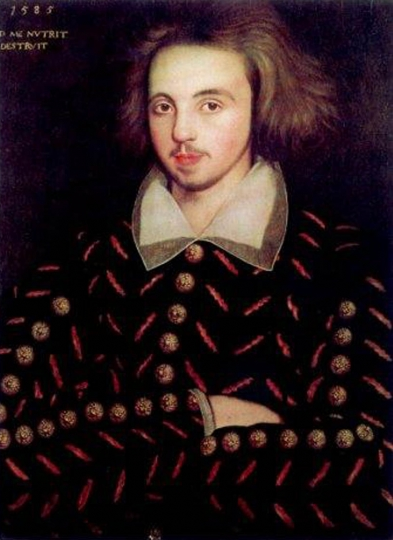
\includegraphics[height = 5 cm]{Marlowe.jpg}
\caption{swag}
\end{figure}

\subsection{Problematisering}
Allt som finns i skafferiet eller kylen kan inte hållas i huvudet. Det leder till att bäst före-datum glöms bort, vilket slutar med att matvaror blir för gamla och måste slängas. Samtidigt gör dålig koll på matvarorna i huset att inköpen blir svåra att planera. Detta innebär att det finns en risk att varor köps in fast de inte behövs. De hinner inte förtäras och blir dåliga. 
\noindent \newline \newline
Rapporten kommer ta upp appens uppbyggnad, dess funktioner och nytta i samhället, lokalt och globalt.


\subsection{Målsättning och syfte}
Skriva en rapport om ett nytt IT-system och beskriva dess tekniska karaktär, samt diskutera runt etiska, samhälleliga och hållbarhetsaspekter. Rapporten är även för att träna användandet av referenser och en introduktion till Urkund. 
\noindent \newline \newline
Målet med appen är att ingen mat ska behöva slängas. Detta genom ett system som fungerar som ett stöd vid planering och inventering av diverse förråd, såsom kylskåpet.

\pagebreak

\section{Resultat}


\subsection{Stora miljöproblemet med den enkla lösningen}
Detta system håller koll på dina matvaror i skafferiet, kylskåpet och frysen. Varorna inventeras i en databas du kan nå med en smartphone. I databasen lagras förutom namnet på varan: kvantitet, inköpsdatum och kategori. Detta gör att du har fullständig koll på matvarorna i hemmet. 
\noindent \newline \newline
Enligt Naturvårdsverket svarar hushåll för den största delen av mängden matavfall i Sverige. I genomsnitt slänger varje person 72 kg mat varje år. Anledningen som ges är en alltför dålig planering, vilket medför svinn. Detta visar sig i form av överinköp, feltolkning av bäst före dag, att alla delar av råvarorna inte används och att tömningen av förpackningar inte görs ordentligt.\cite{Nverket}
\noindent \newline \newline
Appen ska minska mängden slängd mat genom att simplifiera matplaneringen och hålla koll på gamla varor. Användaren kan välja i vilken grad den vill använda systemet. Det går bra att enbart använda det till planering, men det ska också finnas en funktion för att skriva in recept och därigenom beräkna portionspriser. 


\subsection{En lagerarbetare i hemmet}
Den första versionen av systemet kommer enbart vara kopplat till en matvarukedjas kundkort till exempel ICA-kortet. Allt du handlar där förs automatiskt in i databasen och det är sedan upp till dig att kategorisera dem. Det är enbart den första inmatningen av en vara som behöver göras. Sedan kommer det skötas med hjälp av dina tidigare kategoriseringar. Succesivt när du handlar så fylls din databas på och struktureras efter dina preferenser. 
\noindent \newline \newline
Någon gång kommer dock varor ta slut och då ska de flyttas ut ur databasen. Då läser du in varans streckkod med en läsare, vilket leder till att streckkoden kopplas till den scannade varan och plockas ut ur databasen. Den borttagna varan försvinner dock inte helt. Den sparas i en lista, som kan användas vid nästa handling för att lätt se vad som tagit slut.
\noindent \newline \newline
Det finns streckkodsläsare att köpa för hemmet, som kan koppla upp sig mot en dator eller smartphone med Bluetooth för att lätt inventera lager.\cite{Mynewsdesk} Vid många fall kommer dock en streckkodsläsare inte behöva inköpas. I en undersökning från juli 2012 av Flurry har 86 procent av alla svenskar mellan 15 och 64 år en smartphone.\cite{Flurry} En kamera är inkluderat i de flesta smartphones och den kan användas till att läsa streckkoder. Ett exempel är Samsungs Galaxy Round med 13 MP kamera.\cite{NyTeknik} Det finns ett flertal appar som läser streckkoder, såsom Barcode Scanner av ZXing Team och QR BARCODE SCANNER av WB Development Team.\cite{BarcodeScanner, QRBarcodeScanner} 
\noindent \newline \newline
En streckkodsläsare kommer vara inkluderad i appen, men det kommer även finnas möjligheten att ta bort varorna manuellt i listan om användaren skulle föredra det.             
\noindent \newline \newline
Appen kan även arbeta med recept. När ett recept ska matas in skriver användaren ingredienserna och mängden som ska användas, vilket leder till att programmet beräknar portionspris för varorna och maträtten. Det går även att använda streckkodsläsaren för mata in varorna för ett recept. Receptinmatningen är ett verktyg för att hjälpa till med matbudgeten och på ett enkelt sätt visa vilka komponenter i maträtten som är dyrast.        


\subsection{Gör som andra fast bättre}
Det finns flera inventarieprogram på marknaden. En av dem är The Home Food Storage App för iOS. Den låter dig scanna in varorna. Alltså, för varje handling måste du föra in alla varor i systemet. Inköpslista är integrerat och även mål för hur länge varor ska räcka. -Den håller också koll på bäst före-datumet.\cite{FoodStorageApp} 
\noindent \newline \newline
En liknande produkt för smartphones med Android heter Inventory Droid och även den använder sig av telefonens kamera för att skanna streckkoder. Databasen du bygger upp kan lätt exporteras till Excel för lättare bearbetning, vilket gör övergång från smartphone till dator väldigt användarvänligt. Den mer avancerade användaren kan manipulera Exceldokumentet för att beräkna portionspris och dylikt.\cite{InventoryDroid} 


\subsection{Visioner för framtiden}
Appen ska i framtiden samarbeta med de flesta matbutikerna i Sverige. Du ska kunna handla överallt och ändå ha koll på skafferiet hemma. 
\noindent \newline \newline
Findity AB arbetar för att butiker ska lämna ut digitala kvitton som du enkelt har tillgång till genom en smartphone eller dator.\cite{SparaKvittot} Digitalisering av kvitton gör det lättare för den beskrivna appen att spridas, eftersom det då kan baseras på det digitala kvittosystemet.
\noindent \newline \newline
När systemet slagit igenom i Sverige kan det expandera till Europa och sedan världen.            

\pagebreak

\section{Diskussion}
För att appen ska användas krävs det otrolig användarvänlighet. Det får inte vara svårt att manipulera informationen i databasen. Att använda sig av inventerieappar är inte särskilt utspritt och jag tror att det beror på den oerhörda tiden det tar att uppdatera databasen. Den beskrivna appen i rapporten automatiserar det mest tidskrävande steget, vilket är att mata in varor i databasen.
\noindent \newline \newline
Det som krävs för att appen ska bli verklighet är ett samarbete med en stor matvarukedja eller ett vidsträckt system med digitala kvitton. Det som ligger närmast framtiden är förmodligen ett samarbete med en matvarukedja. Tyvärr kan det medföra att matvarukedjan ifråga vill vara unika med systemet och därmed förhindrar spridning, men det kan vara nödvändigt för att få ut appen. Det optimala är en internationell utbredning, vilket skulle medföra att den oerhörda mängden slängd mat skulle minska.
\noindent \newline \newline
Appen är anpassat för moderna smartphones med inbyggd kamera och det är där själva målgruppen finns.  Dock förhindrar detta att systemet får en större spridning i områden utan den levnadsstandarden. De har kanske inte heller samma problem med överinköp. Det är alltså främst  i-länder som är marknaden. 
\noindent \newline \newline
Varje gång man slänger mat så slösar man på ekonomi, miljö och även etik. I-länder slänger mat medan människor i andra länder inte har mat på bordet. Det är inte etiskt rimligt och det är ännu en anledning till varför appen borde finnas. Även om du måste lägga ned tid på att kategorisera databasen från början och ta bort varor ur databasen när de är slut, kan den tiden vara värd det. Då gör du skillnad. 

  


\pagebreak
\begin{thebibliography}{references}

\bibitem{NyTeknik}
Abrahamsson, Håkan. (2013). 	
Koreaner visar upp sin krökta mobil. Nyteknik, 16 oktober, 42, s. 18.

\bibitem{Mynewsdesk}
Amini, Khazar. My News Desk. "Smidig streckkodsläsare löser dina problem". \url{http://www.mynewsdesk.com/se/deltaco-ab/pressreleases/smidig-streckkodslaesare-loeser-dina-problem-876374}.[Hämtad den 2013-10-22].

\bibitem{QRBarcodeScanner}
Google play. WB Development Team. "QR BARCODE SCANNER". \url{https://play.google.com/store/apps/details?id=appinventor.ai_progetto2003.SCAN&hl=sv}[Hämtad den 2013-10-20]

\bibitem{BarcodeScanner}
Google play. ZXing Team. "Barcode Scanner". \url{https://play.google.com/store/apps/details?id=com.google.zxing.client.android&hl=sv}[Hämtad 2013-10-20]

\bibitem{SparaKvittot}
Findity AB. Sparakvittot. "Om Sparakvittot". \url{http://www.sparakvittot.se/om-sparakvittot}[Hämtad 2013-10-22].

\bibitem{Flurry}
Flurry. Flurry Blog. "iOS and Android Adoption Explodes Internationally". \url{http://blog.flurry.com//bid/88867/ios-and-android-adoption-explodes-internationally}[Hämtad den 2013-10-20].

\bibitem{FoodStorageApp}
Long Term Glass Wares LLC. The Home Food Storage App. \url{http://www.foodstorageapp.com/}[Hämtad den 2013-10-19].

\bibitem{InventoryDroid}
RomiSys. Inventory Droid. \url{http://www.romisys.com/pages/inventory-droid.php}.[Hämtad 2013-10-22].
  
\bibitem{Nverket}
Sjöström, Sanna. Naturvårdsverket. "Matsvinn".
\url{http://www.naturvardsverket.se/Miljoarbete-i-samhallet/Miljoarbete-i-Sverige/Uppdelat-efter-omrade/Avfall/Avfallsforebyggande-program/Mat/}[Hämtad den 2013-10-19].





\end{thebibliography}

\end{document}
\documentclass[12pt, a4paper]{article}
\usepackage[swedish]{babel}
\usepackage[utf8]{inputenc}
\usepackage{fullpage}
\usepackage{graphicx}
\usepackage{hyperref}
\usepackage[nottoc,numbib]{tocbibind}
\title{Vad har jag i kylen egentligen?}
\author{Adam Vendelin}


\begin{document}
\maketitle
\begin{center}Uppsala Universitet 
\end{center}
\begin{center}2013-10-24
\end{center}
\pagebreak
\tableofcontents
\pagebreak

\section{Sammanfattning}
\begin{center} \parbox{12cm}{Rapporten behandlar en app som hjälper dig vid inventering av kylskåp och skafferier. Det gör att risken för överinköp minskar, vilket är bra för miljön, ekonomin och även på ett etiskt sätt.  \newline \newline \textit{Nyckelord:}app, databas, inventering, miljö.}
\end{center}
\pagebreak


\section{Introduktion}
\subsection{Bakgrund}
Den här rapporten presenterar en app, utvecklat för att hjälpa människor och miljön. Du ska enkelt kunna se vad som finns i kylskåpet och skafferiet utan att behöva öppna dörrar eller ens vara i huset. Allt detta utan att behöva lägga ned mycket tid på inventeringen. 

\begin{figure}[h!]
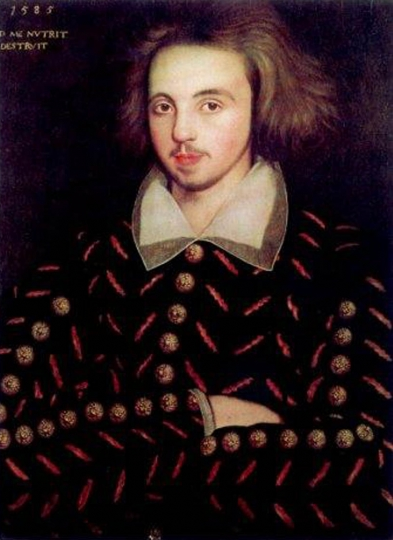
\includegraphics[height = 5 cm]{Marlowe.jpg}
\caption{swag}
\end{figure}

\subsection{Problematisering}
Allt som finns i skafferiet eller kylen kan inte hållas i huvudet. Det leder till att bäst före-datum glöms bort, vilket slutar med att matvaror blir för gamla och måste slängas. Samtidigt gör dålig koll på matvarorna i huset att inköpen blir svåra att planera. Detta innebär att det finns en risk att varor köps in fast de inte behövs. De hinner inte förtäras och blir dåliga. 
\noindent \newline \newline
Rapporten kommer ta upp appens uppbyggnad, dess funktioner och nytta i samhället, lokalt och globalt.


\subsection{Målsättning och syfte}
Skriva en rapport om ett nytt IT-system och beskriva dess tekniska karaktär, samt diskutera runt etiska, samhälleliga och hållbarhetsaspekter. Rapporten är även för att träna användandet av referenser och en introduktion till Urkund. 
\noindent \newline \newline
Målet med appen är att ingen mat ska behöva slängas. Detta genom ett system som fungerar som ett stöd vid planering och inventering av diverse förråd, såsom kylskåpet.

\pagebreak

\section{Resultat}


\subsection{Stora miljöproblemet med den enkla lösningen}
Detta system håller koll på dina matvaror i skafferiet, kylskåpet och frysen. Varorna inventeras i en databas du kan nå med en smartphone. I databasen lagras förutom namnet på varan: kvantitet, inköpsdatum och kategori. Detta gör att du har fullständig koll på matvarorna i hemmet. 
\noindent \newline \newline
Enligt Naturvårdsverket svarar hushåll för den största delen av mängden matavfall i Sverige. I genomsnitt slänger varje person 72 kg mat varje år. Anledningen som ges är en alltför dålig planering, vilket medför svinn. Detta visar sig i form av överinköp, feltolkning av bäst före dag, att alla delar av råvarorna inte används och att tömningen av förpackningar inte görs ordentligt.\cite{Nverket}
\noindent \newline \newline
Appen ska minska mängden slängd mat genom att simplifiera matplaneringen och hålla koll på gamla varor. Användaren kan välja i vilken grad den vill använda systemet. Det går bra att enbart använda det till planering, men det ska också finnas en funktion för att skriva in recept och därigenom beräkna portionspriser. 


\subsection{En lagerarbetare i hemmet}
Den första versionen av systemet kommer enbart vara kopplat till en matvarukedjas kundkort till exempel ICA-kortet. Allt du handlar där förs automatiskt in i databasen och det är sedan upp till dig att kategorisera dem. Det är enbart den första inmatningen av en vara som behöver göras. Sedan kommer det skötas med hjälp av dina tidigare kategoriseringar. Succesivt när du handlar så fylls din databas på och struktureras efter dina preferenser. 
\noindent \newline \newline
Någon gång kommer dock varor ta slut och då ska de flyttas ut ur databasen. Då läser du in varans streckkod med en läsare, vilket leder till att streckkoden kopplas till den scannade varan och plockas ut ur databasen. Den borttagna varan försvinner dock inte helt. Den sparas i en lista, som kan användas vid nästa handling för att lätt se vad som tagit slut.
\noindent \newline \newline
Det finns streckkodsläsare att köpa för hemmet, som kan koppla upp sig mot en dator eller smartphone med Bluetooth för att lätt inventera lager.\cite{Mynewsdesk} Vid många fall kommer dock en streckkodsläsare inte behöva inköpas. I en undersökning från juli 2012 av Flurry har 86 procent av alla svenskar mellan 15 och 64 år en smartphone.\cite{Flurry} En kamera är inkluderat i de flesta smartphones och den kan användas till att läsa streckkoder. Ett exempel är Samsungs Galaxy Round med 13 MP kamera.\cite{NyTeknik} Det finns ett flertal appar som läser streckkoder, såsom Barcode Scanner av ZXing Team och QR BARCODE SCANNER av WB Development Team.\cite{BarcodeScanner, QRBarcodeScanner} 
\noindent \newline \newline
En streckkodsläsare kommer vara inkluderad i appen, men det kommer även finnas möjligheten att ta bort varorna manuellt i listan om användaren skulle föredra det.             
\noindent \newline \newline
Appen kan även arbeta med recept. När ett recept ska matas in skriver användaren ingredienserna och mängden som ska användas, vilket leder till att programmet beräknar portionspris för varorna och maträtten. Det går även att använda streckkodsläsaren för mata in varorna för ett recept. Receptinmatningen är ett verktyg för att hjälpa till med matbudgeten och på ett enkelt sätt visa vilka komponenter i maträtten som är dyrast.        


\subsection{Gör som andra fast bättre}
Det finns flera inventarieprogram på marknaden. En av dem är The Home Food Storage App för iOS. Den låter dig scanna in varorna. Alltså, för varje handling måste du föra in alla varor i systemet. Inköpslista är integrerat och även mål för hur länge varor ska räcka. -Den håller också koll på bäst före-datumet.\cite{FoodStorageApp} 
\noindent \newline \newline
En liknande produkt för smartphones med Android heter Inventory Droid och även den använder sig av telefonens kamera för att skanna streckkoder. Databasen du bygger upp kan lätt exporteras till Excel för lättare bearbetning, vilket gör övergång från smartphone till dator väldigt användarvänligt. Den mer avancerade användaren kan manipulera Exceldokumentet för att beräkna portionspris och dylikt.\cite{InventoryDroid} 


\subsection{Visioner för framtiden}
Appen ska i framtiden samarbeta med de flesta matbutikerna i Sverige. Du ska kunna handla överallt och ändå ha koll på skafferiet hemma. 
\noindent \newline \newline
Findity AB arbetar för att butiker ska lämna ut digitala kvitton som du enkelt har tillgång till genom en smartphone eller dator.\cite{SparaKvittot} Digitalisering av kvitton gör det lättare för den beskrivna appen att spridas, eftersom det då kan baseras på det digitala kvittosystemet.
\noindent \newline \newline
När systemet slagit igenom i Sverige kan det expandera till Europa och sedan världen.            

\pagebreak

\section{Diskussion}
För att appen ska användas krävs det otrolig användarvänlighet. Det får inte vara svårt att manipulera informationen i databasen. Att använda sig av inventerieappar är inte särskilt utspritt och jag tror att det beror på den oerhörda tiden det tar att uppdatera databasen. Den beskrivna appen i rapporten automatiserar det mest tidskrävande steget, vilket är att mata in varor i databasen.
\noindent \newline \newline
Det som krävs för att appen ska bli verklighet är ett samarbete med en stor matvarukedja eller ett vidsträckt system med digitala kvitton. Det som ligger närmast framtiden är förmodligen ett samarbete med en matvarukedja. Tyvärr kan det medföra att matvarukedjan ifråga vill vara unika med systemet och därmed förhindrar spridning, men det kan vara nödvändigt för att få ut appen. Det optimala är en internationell utbredning, vilket skulle medföra att den oerhörda mängden slängd mat skulle minska.
\noindent \newline \newline
Appen är anpassat för moderna smartphones med inbyggd kamera och det är där själva målgruppen finns.  Dock förhindrar detta att systemet får en större spridning i områden utan den levnadsstandarden. De har kanske inte heller samma problem med överinköp. Det är alltså främst  i-länder som är marknaden. 
\noindent \newline \newline
Varje gång man slänger mat så slösar man på ekonomi, miljö och även etik. I-länder slänger mat medan människor i andra länder inte har mat på bordet. Det är inte etiskt rimligt och det är ännu en anledning till varför appen borde finnas. Även om du måste lägga ned tid på att kategorisera databasen från början och ta bort varor ur databasen när de är slut, kan den tiden vara värd det. Då gör du skillnad. 

  


\pagebreak
\begin{thebibliography}{references}

\bibitem{NyTeknik}
Abrahamsson, Håkan. (2013). 	
Koreaner visar upp sin krökta mobil. Nyteknik, 16 oktober, 42, s. 18.

\bibitem{Mynewsdesk}
Amini, Khazar. My News Desk. "Smidig streckkodsläsare löser dina problem". \url{http://www.mynewsdesk.com/se/deltaco-ab/pressreleases/smidig-streckkodslaesare-loeser-dina-problem-876374}.[Hämtad den 2013-10-22].

\bibitem{QRBarcodeScanner}
Google play. WB Development Team. "QR BARCODE SCANNER". \url{https://play.google.com/store/apps/details?id=appinventor.ai_progetto2003.SCAN&hl=sv}[Hämtad den 2013-10-20]

\bibitem{BarcodeScanner}
Google play. ZXing Team. "Barcode Scanner". \url{https://play.google.com/store/apps/details?id=com.google.zxing.client.android&hl=sv}[Hämtad 2013-10-20]

\bibitem{SparaKvittot}
Findity AB. Sparakvittot. "Om Sparakvittot". \url{http://www.sparakvittot.se/om-sparakvittot}[Hämtad 2013-10-22].

\bibitem{Flurry}
Flurry. Flurry Blog. "iOS and Android Adoption Explodes Internationally". \url{http://blog.flurry.com//bid/88867/ios-and-android-adoption-explodes-internationally}[Hämtad den 2013-10-20].

\bibitem{FoodStorageApp}
Long Term Glass Wares LLC. The Home Food Storage App. \url{http://www.foodstorageapp.com/}[Hämtad den 2013-10-19].

\bibitem{InventoryDroid}
RomiSys. Inventory Droid. \url{http://www.romisys.com/pages/inventory-droid.php}.[Hämtad 2013-10-22].
  
\bibitem{Nverket}
Sjöström, Sanna. Naturvårdsverket. "Matsvinn".
\url{http://www.naturvardsverket.se/Miljoarbete-i-samhallet/Miljoarbete-i-Sverige/Uppdelat-efter-omrade/Avfall/Avfallsforebyggande-program/Mat/}[Hämtad den 2013-10-19].





\end{thebibliography}

\end{document}
\documentclass[12pt, a4paper]{article}
\usepackage[swedish]{babel}
\usepackage[utf8]{inputenc}
\usepackage{fullpage}
\usepackage{graphicx}
\usepackage{hyperref}
\usepackage[nottoc,numbib]{tocbibind}
\title{Vad har jag i kylen egentligen?}
\author{Adam Vendelin}


\begin{document}
\maketitle
\begin{center}Uppsala Universitet 
\end{center}
\begin{center}2013-10-24
\end{center}
\pagebreak
\tableofcontents
\pagebreak

\section{Sammanfattning}
\begin{center} \parbox{12cm}{Rapporten behandlar en app som hjälper dig vid inventering av kylskåp och skafferier. Det gör att risken för överinköp minskar, vilket är bra för miljön, ekonomin och även på ett etiskt sätt.  \newline \newline \textit{Nyckelord:}app, databas, inventering, miljö.}
\end{center}
\pagebreak


\section{Introduktion}
\subsection{Bakgrund}
Den här rapporten presenterar en app, utvecklat för att hjälpa människor och miljön. Du ska enkelt kunna se vad som finns i kylskåpet och skafferiet utan att behöva öppna dörrar eller ens vara i huset. Allt detta utan att behöva lägga ned mycket tid på inventeringen. 

\begin{figure}[h!]
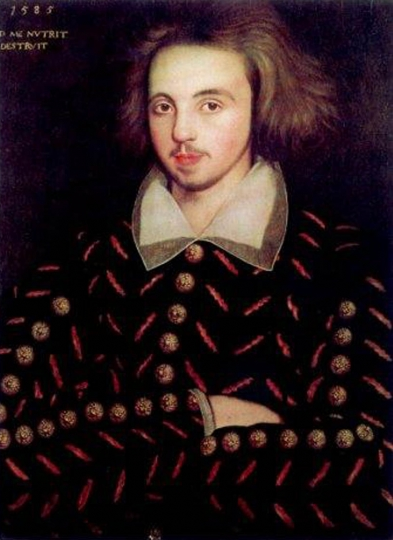
\includegraphics[height = 5 cm]{Marlowe.jpg}
\caption{swag}
\end{figure}

\subsection{Problematisering}
Allt som finns i skafferiet eller kylen kan inte hållas i huvudet. Det leder till att bäst före-datum glöms bort, vilket slutar med att matvaror blir för gamla och måste slängas. Samtidigt gör dålig koll på matvarorna i huset att inköpen blir svåra att planera. Detta innebär att det finns en risk att varor köps in fast de inte behövs. De hinner inte förtäras och blir dåliga. 
\noindent \newline \newline
Rapporten kommer ta upp appens uppbyggnad, dess funktioner och nytta i samhället, lokalt och globalt.


\subsection{Målsättning och syfte}
Skriva en rapport om ett nytt IT-system och beskriva dess tekniska karaktär, samt diskutera runt etiska, samhälleliga och hållbarhetsaspekter. Rapporten är även för att träna användandet av referenser och en introduktion till Urkund. 
\noindent \newline \newline
Målet med appen är att ingen mat ska behöva slängas. Detta genom ett system som fungerar som ett stöd vid planering och inventering av diverse förråd, såsom kylskåpet.

\pagebreak

\section{Resultat}


\subsection{Stora miljöproblemet med den enkla lösningen}
Detta system håller koll på dina matvaror i skafferiet, kylskåpet och frysen. Varorna inventeras i en databas du kan nå med en smartphone. I databasen lagras förutom namnet på varan: kvantitet, inköpsdatum och kategori. Detta gör att du har fullständig koll på matvarorna i hemmet. 
\noindent \newline \newline
Enligt Naturvårdsverket svarar hushåll för den största delen av mängden matavfall i Sverige. I genomsnitt slänger varje person 72 kg mat varje år. Anledningen som ges är en alltför dålig planering, vilket medför svinn. Detta visar sig i form av överinköp, feltolkning av bäst före dag, att alla delar av råvarorna inte används och att tömningen av förpackningar inte görs ordentligt.\cite{Nverket}
\noindent \newline \newline
Appen ska minska mängden slängd mat genom att simplifiera matplaneringen och hålla koll på gamla varor. Användaren kan välja i vilken grad den vill använda systemet. Det går bra att enbart använda det till planering, men det ska också finnas en funktion för att skriva in recept och därigenom beräkna portionspriser. 


\subsection{En lagerarbetare i hemmet}
Den första versionen av systemet kommer enbart vara kopplat till en matvarukedjas kundkort till exempel ICA-kortet. Allt du handlar där förs automatiskt in i databasen och det är sedan upp till dig att kategorisera dem. Det är enbart den första inmatningen av en vara som behöver göras. Sedan kommer det skötas med hjälp av dina tidigare kategoriseringar. Succesivt när du handlar så fylls din databas på och struktureras efter dina preferenser. 
\noindent \newline \newline
Någon gång kommer dock varor ta slut och då ska de flyttas ut ur databasen. Då läser du in varans streckkod med en läsare, vilket leder till att streckkoden kopplas till den scannade varan och plockas ut ur databasen. Den borttagna varan försvinner dock inte helt. Den sparas i en lista, som kan användas vid nästa handling för att lätt se vad som tagit slut.
\noindent \newline \newline
Det finns streckkodsläsare att köpa för hemmet, som kan koppla upp sig mot en dator eller smartphone med Bluetooth för att lätt inventera lager.\cite{Mynewsdesk} Vid många fall kommer dock en streckkodsläsare inte behöva inköpas. I en undersökning från juli 2012 av Flurry har 86 procent av alla svenskar mellan 15 och 64 år en smartphone.\cite{Flurry} En kamera är inkluderat i de flesta smartphones och den kan användas till att läsa streckkoder. Ett exempel är Samsungs Galaxy Round med 13 MP kamera.\cite{NyTeknik} Det finns ett flertal appar som läser streckkoder, såsom Barcode Scanner av ZXing Team och QR BARCODE SCANNER av WB Development Team.\cite{BarcodeScanner, QRBarcodeScanner} 
\noindent \newline \newline
En streckkodsläsare kommer vara inkluderad i appen, men det kommer även finnas möjligheten att ta bort varorna manuellt i listan om användaren skulle föredra det.             
\noindent \newline \newline
Appen kan även arbeta med recept. När ett recept ska matas in skriver användaren ingredienserna och mängden som ska användas, vilket leder till att programmet beräknar portionspris för varorna och maträtten. Det går även att använda streckkodsläsaren för mata in varorna för ett recept. Receptinmatningen är ett verktyg för att hjälpa till med matbudgeten och på ett enkelt sätt visa vilka komponenter i maträtten som är dyrast.        


\subsection{Gör som andra fast bättre}
Det finns flera inventarieprogram på marknaden. En av dem är The Home Food Storage App för iOS. Den låter dig scanna in varorna. Alltså, för varje handling måste du föra in alla varor i systemet. Inköpslista är integrerat och även mål för hur länge varor ska räcka. -Den håller också koll på bäst före-datumet.\cite{FoodStorageApp} 
\noindent \newline \newline
En liknande produkt för smartphones med Android heter Inventory Droid och även den använder sig av telefonens kamera för att skanna streckkoder. Databasen du bygger upp kan lätt exporteras till Excel för lättare bearbetning, vilket gör övergång från smartphone till dator väldigt användarvänligt. Den mer avancerade användaren kan manipulera Exceldokumentet för att beräkna portionspris och dylikt.\cite{InventoryDroid} 


\subsection{Visioner för framtiden}
Appen ska i framtiden samarbeta med de flesta matbutikerna i Sverige. Du ska kunna handla överallt och ändå ha koll på skafferiet hemma. 
\noindent \newline \newline
Findity AB arbetar för att butiker ska lämna ut digitala kvitton som du enkelt har tillgång till genom en smartphone eller dator.\cite{SparaKvittot} Digitalisering av kvitton gör det lättare för den beskrivna appen att spridas, eftersom det då kan baseras på det digitala kvittosystemet.
\noindent \newline \newline
När systemet slagit igenom i Sverige kan det expandera till Europa och sedan världen.            

\pagebreak

\section{Diskussion}
För att appen ska användas krävs det otrolig användarvänlighet. Det får inte vara svårt att manipulera informationen i databasen. Att använda sig av inventerieappar är inte särskilt utspritt och jag tror att det beror på den oerhörda tiden det tar att uppdatera databasen. Den beskrivna appen i rapporten automatiserar det mest tidskrävande steget, vilket är att mata in varor i databasen.
\noindent \newline \newline
Det som krävs för att appen ska bli verklighet är ett samarbete med en stor matvarukedja eller ett vidsträckt system med digitala kvitton. Det som ligger närmast framtiden är förmodligen ett samarbete med en matvarukedja. Tyvärr kan det medföra att matvarukedjan ifråga vill vara unika med systemet och därmed förhindrar spridning, men det kan vara nödvändigt för att få ut appen. Det optimala är en internationell utbredning, vilket skulle medföra att den oerhörda mängden slängd mat skulle minska.
\noindent \newline \newline
Appen är anpassat för moderna smartphones med inbyggd kamera och det är där själva målgruppen finns.  Dock förhindrar detta att systemet får en större spridning i områden utan den levnadsstandarden. De har kanske inte heller samma problem med överinköp. Det är alltså främst  i-länder som är marknaden. 
\noindent \newline \newline
Varje gång man slänger mat så slösar man på ekonomi, miljö och även etik. I-länder slänger mat medan människor i andra länder inte har mat på bordet. Det är inte etiskt rimligt och det är ännu en anledning till varför appen borde finnas. Även om du måste lägga ned tid på att kategorisera databasen från början och ta bort varor ur databasen när de är slut, kan den tiden vara värd det. Då gör du skillnad. 

  


\pagebreak
\begin{thebibliography}{references}

\bibitem{NyTeknik}
Abrahamsson, Håkan. (2013). 	
Koreaner visar upp sin krökta mobil. Nyteknik, 16 oktober, 42, s. 18.

\bibitem{Mynewsdesk}
Amini, Khazar. My News Desk. "Smidig streckkodsläsare löser dina problem". \url{http://www.mynewsdesk.com/se/deltaco-ab/pressreleases/smidig-streckkodslaesare-loeser-dina-problem-876374}.[Hämtad den 2013-10-22].

\bibitem{QRBarcodeScanner}
Google play. WB Development Team. "QR BARCODE SCANNER". \url{https://play.google.com/store/apps/details?id=appinventor.ai_progetto2003.SCAN&hl=sv}[Hämtad den 2013-10-20]

\bibitem{BarcodeScanner}
Google play. ZXing Team. "Barcode Scanner". \url{https://play.google.com/store/apps/details?id=com.google.zxing.client.android&hl=sv}[Hämtad 2013-10-20]

\bibitem{SparaKvittot}
Findity AB. Sparakvittot. "Om Sparakvittot". \url{http://www.sparakvittot.se/om-sparakvittot}[Hämtad 2013-10-22].

\bibitem{Flurry}
Flurry. Flurry Blog. "iOS and Android Adoption Explodes Internationally". \url{http://blog.flurry.com//bid/88867/ios-and-android-adoption-explodes-internationally}[Hämtad den 2013-10-20].

\bibitem{FoodStorageApp}
Long Term Glass Wares LLC. The Home Food Storage App. \url{http://www.foodstorageapp.com/}[Hämtad den 2013-10-19].

\bibitem{InventoryDroid}
RomiSys. Inventory Droid. \url{http://www.romisys.com/pages/inventory-droid.php}.[Hämtad 2013-10-22].
  
\bibitem{Nverket}
Sjöström, Sanna. Naturvårdsverket. "Matsvinn".
\url{http://www.naturvardsverket.se/Miljoarbete-i-samhallet/Miljoarbete-i-Sverige/Uppdelat-efter-omrade/Avfall/Avfallsforebyggande-program/Mat/}[Hämtad den 2013-10-19].





\end{thebibliography}

\end{document}
\documentclass[12pt, a4paper]{article}
\usepackage[swedish]{babel}
\usepackage[utf8]{inputenc}
\usepackage{fullpage}
\usepackage{graphicx}
\usepackage{hyperref}
\usepackage[nottoc,numbib]{tocbibind}
\title{Vad har jag i kylen egentligen?}
\author{Adam Vendelin}


\begin{document}
\maketitle
\begin{center}Uppsala Universitet 
\end{center}
\begin{center}2013-10-24
\end{center}
\pagebreak
\tableofcontents
\pagebreak

\section{Sammanfattning}
\begin{center} \parbox{12cm}{Rapporten behandlar en app som hjälper dig vid inventering av kylskåp och skafferier. Det gör att risken för överinköp minskar, vilket är bra för miljön, ekonomin och även på ett etiskt sätt.  \newline \newline \textit{Nyckelord:}app, databas, inventering, miljö.}
\end{center}
\pagebreak


\section{Introduktion}
\subsection{Bakgrund}
Den här rapporten presenterar en app, utvecklat för att hjälpa människor och miljön. Du ska enkelt kunna se vad som finns i kylskåpet och skafferiet utan att behöva öppna dörrar eller ens vara i huset. Allt detta utan att behöva lägga ned mycket tid på inventeringen. 

\begin{figure}[h!]
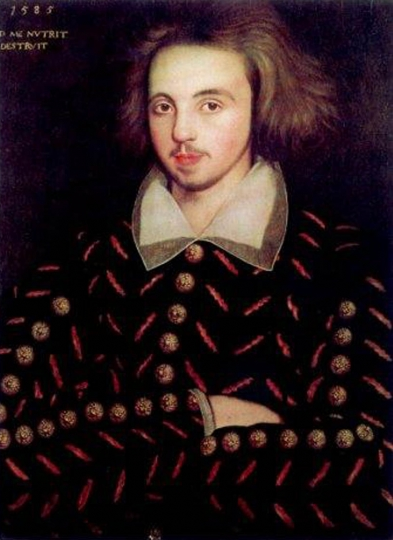
\includegraphics[height = 5 cm]{Marlowe.jpg}
\caption{swag}
\end{figure}

\subsection{Problematisering}
Allt som finns i skafferiet eller kylen kan inte hållas i huvudet. Det leder till att bäst före-datum glöms bort, vilket slutar med att matvaror blir för gamla och måste slängas. Samtidigt gör dålig koll på matvarorna i huset att inköpen blir svåra att planera. Detta innebär att det finns en risk att varor köps in fast de inte behövs. De hinner inte förtäras och blir dåliga. 
\noindent \newline \newline
Rapporten kommer ta upp appens uppbyggnad, dess funktioner och nytta i samhället, lokalt och globalt.


\subsection{Målsättning och syfte}
Skriva en rapport om ett nytt IT-system och beskriva dess tekniska karaktär, samt diskutera runt etiska, samhälleliga och hållbarhetsaspekter. Rapporten är även för att träna användandet av referenser och en introduktion till Urkund. 
\noindent \newline \newline
Målet med appen är att ingen mat ska behöva slängas. Detta genom ett system som fungerar som ett stöd vid planering och inventering av diverse förråd, såsom kylskåpet.

\pagebreak

\section{Resultat}


\subsection{Stora miljöproblemet med den enkla lösningen}
Detta system håller koll på dina matvaror i skafferiet, kylskåpet och frysen. Varorna inventeras i en databas du kan nå med en smartphone. I databasen lagras förutom namnet på varan: kvantitet, inköpsdatum och kategori. Detta gör att du har fullständig koll på matvarorna i hemmet. 
\noindent \newline \newline
Enligt Naturvårdsverket svarar hushåll för den största delen av mängden matavfall i Sverige. I genomsnitt slänger varje person 72 kg mat varje år. Anledningen som ges är en alltför dålig planering, vilket medför svinn. Detta visar sig i form av överinköp, feltolkning av bäst före dag, att alla delar av råvarorna inte används och att tömningen av förpackningar inte görs ordentligt.\cite{Nverket}
\noindent \newline \newline
Appen ska minska mängden slängd mat genom att simplifiera matplaneringen och hålla koll på gamla varor. Användaren kan välja i vilken grad den vill använda systemet. Det går bra att enbart använda det till planering, men det ska också finnas en funktion för att skriva in recept och därigenom beräkna portionspriser. 


\subsection{En lagerarbetare i hemmet}
Den första versionen av systemet kommer enbart vara kopplat till en matvarukedjas kundkort till exempel ICA-kortet. Allt du handlar där förs automatiskt in i databasen och det är sedan upp till dig att kategorisera dem. Det är enbart den första inmatningen av en vara som behöver göras. Sedan kommer det skötas med hjälp av dina tidigare kategoriseringar. Succesivt när du handlar så fylls din databas på och struktureras efter dina preferenser. 
\noindent \newline \newline
Någon gång kommer dock varor ta slut och då ska de flyttas ut ur databasen. Då läser du in varans streckkod med en läsare, vilket leder till att streckkoden kopplas till den scannade varan och plockas ut ur databasen. Den borttagna varan försvinner dock inte helt. Den sparas i en lista, som kan användas vid nästa handling för att lätt se vad som tagit slut.
\noindent \newline \newline
Det finns streckkodsläsare att köpa för hemmet, som kan koppla upp sig mot en dator eller smartphone med Bluetooth för att lätt inventera lager.\cite{Mynewsdesk} Vid många fall kommer dock en streckkodsläsare inte behöva inköpas. I en undersökning från juli 2012 av Flurry har 86 procent av alla svenskar mellan 15 och 64 år en smartphone.\cite{Flurry} En kamera är inkluderat i de flesta smartphones och den kan användas till att läsa streckkoder. Ett exempel är Samsungs Galaxy Round med 13 MP kamera.\cite{NyTeknik} Det finns ett flertal appar som läser streckkoder, såsom Barcode Scanner av ZXing Team och QR BARCODE SCANNER av WB Development Team.\cite{BarcodeScanner, QRBarcodeScanner} 
\noindent \newline \newline
En streckkodsläsare kommer vara inkluderad i appen, men det kommer även finnas möjligheten att ta bort varorna manuellt i listan om användaren skulle föredra det.             
\noindent \newline \newline
Appen kan även arbeta med recept. När ett recept ska matas in skriver användaren ingredienserna och mängden som ska användas, vilket leder till att programmet beräknar portionspris för varorna och maträtten. Det går även att använda streckkodsläsaren för mata in varorna för ett recept. Receptinmatningen är ett verktyg för att hjälpa till med matbudgeten och på ett enkelt sätt visa vilka komponenter i maträtten som är dyrast.        


\subsection{Gör som andra fast bättre}
Det finns flera inventarieprogram på marknaden. En av dem är The Home Food Storage App för iOS. Den låter dig scanna in varorna. Alltså, för varje handling måste du föra in alla varor i systemet. Inköpslista är integrerat och även mål för hur länge varor ska räcka. -Den håller också koll på bäst före-datumet.\cite{FoodStorageApp} 
\noindent \newline \newline
En liknande produkt för smartphones med Android heter Inventory Droid och även den använder sig av telefonens kamera för att skanna streckkoder. Databasen du bygger upp kan lätt exporteras till Excel för lättare bearbetning, vilket gör övergång från smartphone till dator väldigt användarvänligt. Den mer avancerade användaren kan manipulera Exceldokumentet för att beräkna portionspris och dylikt.\cite{InventoryDroid} 


\subsection{Visioner för framtiden}
Appen ska i framtiden samarbeta med de flesta matbutikerna i Sverige. Du ska kunna handla överallt och ändå ha koll på skafferiet hemma. 
\noindent \newline \newline
Findity AB arbetar för att butiker ska lämna ut digitala kvitton som du enkelt har tillgång till genom en smartphone eller dator.\cite{SparaKvittot} Digitalisering av kvitton gör det lättare för den beskrivna appen att spridas, eftersom det då kan baseras på det digitala kvittosystemet.
\noindent \newline \newline
När systemet slagit igenom i Sverige kan det expandera till Europa och sedan världen.            

\pagebreak

\section{Diskussion}
För att appen ska användas krävs det otrolig användarvänlighet. Det får inte vara svårt att manipulera informationen i databasen. Att använda sig av inventerieappar är inte särskilt utspritt och jag tror att det beror på den oerhörda tiden det tar att uppdatera databasen. Den beskrivna appen i rapporten automatiserar det mest tidskrävande steget, vilket är att mata in varor i databasen.
\noindent \newline \newline
Det som krävs för att appen ska bli verklighet är ett samarbete med en stor matvarukedja eller ett vidsträckt system med digitala kvitton. Det som ligger närmast framtiden är förmodligen ett samarbete med en matvarukedja. Tyvärr kan det medföra att matvarukedjan ifråga vill vara unika med systemet och därmed förhindrar spridning, men det kan vara nödvändigt för att få ut appen. Det optimala är en internationell utbredning, vilket skulle medföra att den oerhörda mängden slängd mat skulle minska.
\noindent \newline \newline
Appen är anpassat för moderna smartphones med inbyggd kamera och det är där själva målgruppen finns.  Dock förhindrar detta att systemet får en större spridning i områden utan den levnadsstandarden. De har kanske inte heller samma problem med överinköp. Det är alltså främst  i-länder som är marknaden. 
\noindent \newline \newline
Varje gång man slänger mat så slösar man på ekonomi, miljö och även etik. I-länder slänger mat medan människor i andra länder inte har mat på bordet. Det är inte etiskt rimligt och det är ännu en anledning till varför appen borde finnas. Även om du måste lägga ned tid på att kategorisera databasen från början och ta bort varor ur databasen när de är slut, kan den tiden vara värd det. Då gör du skillnad. 

  


\pagebreak
\begin{thebibliography}{references}

\bibitem{NyTeknik}
Abrahamsson, Håkan. (2013). 	
Koreaner visar upp sin krökta mobil. Nyteknik, 16 oktober, 42, s. 18.

\bibitem{Mynewsdesk}
Amini, Khazar. My News Desk. "Smidig streckkodsläsare löser dina problem". \url{http://www.mynewsdesk.com/se/deltaco-ab/pressreleases/smidig-streckkodslaesare-loeser-dina-problem-876374}.[Hämtad den 2013-10-22].

\bibitem{QRBarcodeScanner}
Google play. WB Development Team. "QR BARCODE SCANNER". \url{https://play.google.com/store/apps/details?id=appinventor.ai_progetto2003.SCAN&hl=sv}[Hämtad den 2013-10-20]

\bibitem{BarcodeScanner}
Google play. ZXing Team. "Barcode Scanner". \url{https://play.google.com/store/apps/details?id=com.google.zxing.client.android&hl=sv}[Hämtad 2013-10-20]

\bibitem{SparaKvittot}
Findity AB. Sparakvittot. "Om Sparakvittot". \url{http://www.sparakvittot.se/om-sparakvittot}[Hämtad 2013-10-22].

\bibitem{Flurry}
Flurry. Flurry Blog. "iOS and Android Adoption Explodes Internationally". \url{http://blog.flurry.com//bid/88867/ios-and-android-adoption-explodes-internationally}[Hämtad den 2013-10-20].

\bibitem{FoodStorageApp}
Long Term Glass Wares LLC. The Home Food Storage App. \url{http://www.foodstorageapp.com/}[Hämtad den 2013-10-19].

\bibitem{InventoryDroid}
RomiSys. Inventory Droid. \url{http://www.romisys.com/pages/inventory-droid.php}.[Hämtad 2013-10-22].
  
\bibitem{Nverket}
Sjöström, Sanna. Naturvårdsverket. "Matsvinn".
\url{http://www.naturvardsverket.se/Miljoarbete-i-samhallet/Miljoarbete-i-Sverige/Uppdelat-efter-omrade/Avfall/Avfallsforebyggande-program/Mat/}[Hämtad den 2013-10-19].





\end{thebibliography}

\end{document}
\documentclass[12pt, a4paper]{article}
\usepackage[swedish]{babel}
\usepackage[utf8]{inputenc}
\usepackage{fullpage}
\usepackage{graphicx}
\usepackage{hyperref}
\usepackage[nottoc,numbib]{tocbibind}
\title{Vad har jag i kylen egentligen?}
\author{Adam Vendelin}


\begin{document}
\maketitle
\begin{center}Uppsala Universitet 
\end{center}
\begin{center}2013-10-24
\end{center}
\pagebreak
\tableofcontents
\pagebreak

\section{Sammanfattning}
\begin{center} \parbox{12cm}{Rapporten behandlar en app som hjälper dig vid inventering av kylskåp och skafferier. Det gör att risken för överinköp minskar, vilket är bra för miljön, ekonomin och även på ett etiskt sätt.  \newline \newline \textit{Nyckelord:}app, databas, inventering, miljö.}
\end{center}
\pagebreak


\section{Introduktion}
\subsection{Bakgrund}
Den här rapporten presenterar en app, utvecklat för att hjälpa människor och miljön. Du ska enkelt kunna se vad som finns i kylskåpet och skafferiet utan att behöva öppna dörrar eller ens vara i huset. Allt detta utan att behöva lägga ned mycket tid på inventeringen. 

\begin{figure}[h!]
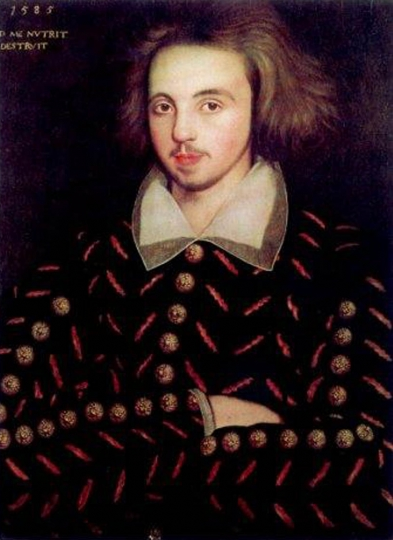
\includegraphics[height = 5 cm]{Marlowe.jpg}
\caption{swag}
\end{figure}

\subsection{Problematisering}
Allt som finns i skafferiet eller kylen kan inte hållas i huvudet. Det leder till att bäst före-datum glöms bort, vilket slutar med att matvaror blir för gamla och måste slängas. Samtidigt gör dålig koll på matvarorna i huset att inköpen blir svåra att planera. Detta innebär att det finns en risk att varor köps in fast de inte behövs. De hinner inte förtäras och blir dåliga. 
\noindent \newline \newline
Rapporten kommer ta upp appens uppbyggnad, dess funktioner och nytta i samhället, lokalt och globalt.


\subsection{Målsättning och syfte}
Skriva en rapport om ett nytt IT-system och beskriva dess tekniska karaktär, samt diskutera runt etiska, samhälleliga och hållbarhetsaspekter. Rapporten är även för att träna användandet av referenser och en introduktion till Urkund. 
\noindent \newline \newline
Målet med appen är att ingen mat ska behöva slängas. Detta genom ett system som fungerar som ett stöd vid planering och inventering av diverse förråd, såsom kylskåpet.

\pagebreak

\section{Resultat}


\subsection{Stora miljöproblemet med den enkla lösningen}
Detta system håller koll på dina matvaror i skafferiet, kylskåpet och frysen. Varorna inventeras i en databas du kan nå med en smartphone. I databasen lagras förutom namnet på varan: kvantitet, inköpsdatum och kategori. Detta gör att du har fullständig koll på matvarorna i hemmet. 
\noindent \newline \newline
Enligt Naturvårdsverket svarar hushåll för den största delen av mängden matavfall i Sverige. I genomsnitt slänger varje person 72 kg mat varje år. Anledningen som ges är en alltför dålig planering, vilket medför svinn. Detta visar sig i form av överinköp, feltolkning av bäst före dag, att alla delar av råvarorna inte används och att tömningen av förpackningar inte görs ordentligt.\cite{Nverket}
\noindent \newline \newline
Appen ska minska mängden slängd mat genom att simplifiera matplaneringen och hålla koll på gamla varor. Användaren kan välja i vilken grad den vill använda systemet. Det går bra att enbart använda det till planering, men det ska också finnas en funktion för att skriva in recept och därigenom beräkna portionspriser. 


\subsection{En lagerarbetare i hemmet}
Den första versionen av systemet kommer enbart vara kopplat till en matvarukedjas kundkort till exempel ICA-kortet. Allt du handlar där förs automatiskt in i databasen och det är sedan upp till dig att kategorisera dem. Det är enbart den första inmatningen av en vara som behöver göras. Sedan kommer det skötas med hjälp av dina tidigare kategoriseringar. Succesivt när du handlar så fylls din databas på och struktureras efter dina preferenser. 
\noindent \newline \newline
Någon gång kommer dock varor ta slut och då ska de flyttas ut ur databasen. Då läser du in varans streckkod med en läsare, vilket leder till att streckkoden kopplas till den scannade varan och plockas ut ur databasen. Den borttagna varan försvinner dock inte helt. Den sparas i en lista, som kan användas vid nästa handling för att lätt se vad som tagit slut.
\noindent \newline \newline
Det finns streckkodsläsare att köpa för hemmet, som kan koppla upp sig mot en dator eller smartphone med Bluetooth för att lätt inventera lager.\cite{Mynewsdesk} Vid många fall kommer dock en streckkodsläsare inte behöva inköpas. I en undersökning från juli 2012 av Flurry har 86 procent av alla svenskar mellan 15 och 64 år en smartphone.\cite{Flurry} En kamera är inkluderat i de flesta smartphones och den kan användas till att läsa streckkoder. Ett exempel är Samsungs Galaxy Round med 13 MP kamera.\cite{NyTeknik} Det finns ett flertal appar som läser streckkoder, såsom Barcode Scanner av ZXing Team och QR BARCODE SCANNER av WB Development Team.\cite{BarcodeScanner, QRBarcodeScanner} 
\noindent \newline \newline
En streckkodsläsare kommer vara inkluderad i appen, men det kommer även finnas möjligheten att ta bort varorna manuellt i listan om användaren skulle föredra det.             
\noindent \newline \newline
Appen kan även arbeta med recept. När ett recept ska matas in skriver användaren ingredienserna och mängden som ska användas, vilket leder till att programmet beräknar portionspris för varorna och maträtten. Det går även att använda streckkodsläsaren för mata in varorna för ett recept. Receptinmatningen är ett verktyg för att hjälpa till med matbudgeten och på ett enkelt sätt visa vilka komponenter i maträtten som är dyrast.        


\subsection{Gör som andra fast bättre}
Det finns flera inventarieprogram på marknaden. En av dem är The Home Food Storage App för iOS. Den låter dig scanna in varorna. Alltså, för varje handling måste du föra in alla varor i systemet. Inköpslista är integrerat och även mål för hur länge varor ska räcka. -Den håller också koll på bäst före-datumet.\cite{FoodStorageApp} 
\noindent \newline \newline
En liknande produkt för smartphones med Android heter Inventory Droid och även den använder sig av telefonens kamera för att skanna streckkoder. Databasen du bygger upp kan lätt exporteras till Excel för lättare bearbetning, vilket gör övergång från smartphone till dator väldigt användarvänligt. Den mer avancerade användaren kan manipulera Exceldokumentet för att beräkna portionspris och dylikt.\cite{InventoryDroid} 


\subsection{Visioner för framtiden}
Appen ska i framtiden samarbeta med de flesta matbutikerna i Sverige. Du ska kunna handla överallt och ändå ha koll på skafferiet hemma. 
\noindent \newline \newline
Findity AB arbetar för att butiker ska lämna ut digitala kvitton som du enkelt har tillgång till genom en smartphone eller dator.\cite{SparaKvittot} Digitalisering av kvitton gör det lättare för den beskrivna appen att spridas, eftersom det då kan baseras på det digitala kvittosystemet.
\noindent \newline \newline
När systemet slagit igenom i Sverige kan det expandera till Europa och sedan världen.            

\pagebreak

\section{Diskussion}
För att appen ska användas krävs det otrolig användarvänlighet. Det får inte vara svårt att manipulera informationen i databasen. Att använda sig av inventerieappar är inte särskilt utspritt och jag tror att det beror på den oerhörda tiden det tar att uppdatera databasen. Den beskrivna appen i rapporten automatiserar det mest tidskrävande steget, vilket är att mata in varor i databasen.
\noindent \newline \newline
Det som krävs för att appen ska bli verklighet är ett samarbete med en stor matvarukedja eller ett vidsträckt system med digitala kvitton. Det som ligger närmast framtiden är förmodligen ett samarbete med en matvarukedja. Tyvärr kan det medföra att matvarukedjan ifråga vill vara unika med systemet och därmed förhindrar spridning, men det kan vara nödvändigt för att få ut appen. Det optimala är en internationell utbredning, vilket skulle medföra att den oerhörda mängden slängd mat skulle minska.
\noindent \newline \newline
Appen är anpassat för moderna smartphones med inbyggd kamera och det är där själva målgruppen finns.  Dock förhindrar detta att systemet får en större spridning i områden utan den levnadsstandarden. De har kanske inte heller samma problem med överinköp. Det är alltså främst  i-länder som är marknaden. 
\noindent \newline \newline
Varje gång man slänger mat så slösar man på ekonomi, miljö och även etik. I-länder slänger mat medan människor i andra länder inte har mat på bordet. Det är inte etiskt rimligt och det är ännu en anledning till varför appen borde finnas. Även om du måste lägga ned tid på att kategorisera databasen från början och ta bort varor ur databasen när de är slut, kan den tiden vara värd det. Då gör du skillnad. 

  


\pagebreak
\begin{thebibliography}{references}

\bibitem{NyTeknik}
Abrahamsson, Håkan. (2013). 	
Koreaner visar upp sin krökta mobil. Nyteknik, 16 oktober, 42, s. 18.

\bibitem{Mynewsdesk}
Amini, Khazar. My News Desk. "Smidig streckkodsläsare löser dina problem". \url{http://www.mynewsdesk.com/se/deltaco-ab/pressreleases/smidig-streckkodslaesare-loeser-dina-problem-876374}.[Hämtad den 2013-10-22].

\bibitem{QRBarcodeScanner}
Google play. WB Development Team. "QR BARCODE SCANNER". \url{https://play.google.com/store/apps/details?id=appinventor.ai_progetto2003.SCAN&hl=sv}[Hämtad den 2013-10-20]

\bibitem{BarcodeScanner}
Google play. ZXing Team. "Barcode Scanner". \url{https://play.google.com/store/apps/details?id=com.google.zxing.client.android&hl=sv}[Hämtad 2013-10-20]

\bibitem{SparaKvittot}
Findity AB. Sparakvittot. "Om Sparakvittot". \url{http://www.sparakvittot.se/om-sparakvittot}[Hämtad 2013-10-22].

\bibitem{Flurry}
Flurry. Flurry Blog. "iOS and Android Adoption Explodes Internationally". \url{http://blog.flurry.com//bid/88867/ios-and-android-adoption-explodes-internationally}[Hämtad den 2013-10-20].

\bibitem{FoodStorageApp}
Long Term Glass Wares LLC. The Home Food Storage App. \url{http://www.foodstorageapp.com/}[Hämtad den 2013-10-19].

\bibitem{InventoryDroid}
RomiSys. Inventory Droid. \url{http://www.romisys.com/pages/inventory-droid.php}.[Hämtad 2013-10-22].
  
\bibitem{Nverket}
Sjöström, Sanna. Naturvårdsverket. "Matsvinn".
\url{http://www.naturvardsverket.se/Miljoarbete-i-samhallet/Miljoarbete-i-Sverige/Uppdelat-efter-omrade/Avfall/Avfallsforebyggande-program/Mat/}[Hämtad den 2013-10-19].





\end{thebibliography}

\end{document}

